\documentclass[11pt,a4paper]{article}
\frenchspacing
\usepackage[margin=22mm]{geometry}
\usepackage{amsmath,amssymb}
\usepackage{booktabs,tabularx,array}
\usepackage{tikz}
\usetikzlibrary{arrows.meta,positioning,shapes.geometric}
\usepackage[hidelinks]{hyperref}
\usepackage{xcolor}
\usepackage[affil-it]{authblk}
\setlength{\parskip}{4pt}
\setlength{\emergencystretch}{2em}

\newcommand{\st}[1]{\textsc{#1}}
\newcommand{\file}[1]{\texttt{#1}}

\title{The Pathfinder engine\\ {\small\file{github.com/vd1/pathfinder}}}

\author[1]{Vincent Danos}
\author[2,3]{Elham Kashefi}
\author[3]{William Waites}
\affil[1]{CNRS, ENS}
\affil[2]{CNRS, LIP6}
\affil[3]{University of Edinburgh}

\date{16 September 2026}

\begin{document}
\maketitle

\begin{abstract}
Pathfinder is an ``AI for science'' research program aiming a creating new
research ideas at scale. Its engine scans and scores pairs
from selected corpora for scientific
connexions and attempts at developing the most promising into publishable notes
which human experts can evaluate.\footnote{Eventually, in a world where agents
dominate the scientific throughput, a publication-looking output may not be the
better format; but that seems appropriate at the moment for a hybrid AI/human
led research process.} No human is required during the process once the initial
corpora and score threshold for eligibility are set up. Given a pair of papers with a potentially
interesting connexion, the engine launches a team of AI agents to produce a
research note. The note is then submitted to an agent verifier who
decides whether to elaborate it into a publication output for external
assessment.

In this note we describe the Pathfinder engine as a state transition system
at a level of details suitable
for human and AI readers, so they can jointly and easily re-implement it, should
they wish to, and adjust it to their specific needs.
\end{abstract}

\section{The Pathfinder program}
Pathfinder takes two corpora of scientific papers, concretely arXiv deposits,
\(Q\) and \(P\), and, using AI agents (currently using OpenAI and Anthropic
models), looks for pairs \((q,p)\in Q\times P\) with an interesting enough
connexion to try to elaborate it as a pre-publication. Ideally, the
pre-publication satisfies the usual constraints of correctness, novelty,
relevance, readability, and exposition of related work. In some cases the pair
is supplemented with a seed note describing the putative connexion, supplied by
the agent that scanned and scored the pair. The seed is a starting point, not a
claim the researcher agents should support.

Pathfinder is concerned with finding questions and connexions, rather than
solving a conjecture fixed in advance. This is not a new idea. Swanson's
\emph{undiscovered public knowledge} concerns implications that become visible
when previously separate published findings are brought together
\cite{swanson1986}. Gentner's account of analogy emphasises correspondences
between relationships, rather than superficial resemblance \cite{gentner1983}.
This offers one way to understand Pathfinder's search: a useful connexion
may transfer an argument or mechanism between settings whose objects look
quite different. The research phase must then establish whether that
transfer is justified. What
is new is that AI agents are now available that can plausibly stand in for human
experts and search this space at scale. Whether the systematic search for connexions
leads to useful scientific knowledge can now be tested. Pathfinder is a first step
in this direction.

% \subsection{Object of this note}
The goal of this note is to specify Pathfinder at a level sufficient for an
agent or a human programmer to reimplement the protocol, without prescribing
every detail of its present implementation.

% The experiment describes the setup, the observed
% outcomes, and selected scientific results; internal acceptance is distinguished
% from evidence of validity and novelty.

% Some may already have been discussed elsewhere, without a direct citation
% between the papers. The aim is not just to find similar articles, but to
% discover what putting them together allows us to ask or understand.

% This type of task is commonly carried out by human experts. A question in a
% seminar can supply the seed of an idea connecting different bodies of work; in
% favourable circumstances it is pursued all the way to a publication. Agents
% allow such attempts to be made concurrently and under explicit resource
% limits. The purpose is to explore more candidate connexions, not to assume
% that breadth replaces scientific judgement.




% Thus the research phase is a sampler. Its verdict concerns the investigation
% actually carried out, not all possible connexions between the pair. A fresh
% run ending in \st{pause} does not withdraw a result established by a different
% run. Reassessing that result requires supplying it as the object of review.
% Independent reruns must therefore keep separate records.


% Before we give examples two comparisons between Pathfinder
% and existing practices may be useful.

How do human experts get new ideas? It happens sometimes through seminars. The
seed of an idea is provided by someone in the audience, and a connexion made,
which, in favourable circumstances, can lead to a publication. By using modern
agents (which are competent experts on every corpus, and always ``willing'' to
contribute), one can do it faster, cheaper, and, therefore, at a larger scale.
We have ran Pathfinder on sets of paper of size about a hundred each for a
reasonable token budget (for budget related considerations \S\ref{eq:pilot-boundary}).

Another comparison is with word embeddings and the idea that what a
word means can be seen from the company it keeps. A scientific paper can likewise be
understood through other papers to which it can be related: work that may
use its methods, extend its results, or challenge its assumptions. Citations
record the past connexions. Pathfinder looks at possible ones. Its scan
proposes links that the citation graph does not show; its research phase tries
to establish what those links mean and whether they yield anything useful.

\section{The 10-by-10 experiment}
\label{sec:pilot}

% The outcomes below are those of the saved campaign. They provide examples of
% what the protocol can produce and of where it stops; they do not estimate a
% general discovery rate.

% \subsection{Setup and experimental record}
To test the engine on a small scale,
we picked the ten most recent Arxiv papers (at the time of the call)
returned by arxiv for the
queries ``mechanism design'' (for $Q$) and ``agentic cooperation'' (for $P$). These
papers are labelled $Q1,\ldots,Q10$ and $P1,\ldots,P10$. The $Q$-collection includes
economic mechanisms, learning-augmented algorithms, robotic hardware, and
astronomical instrumentation. The $P$ one includes multi-agent learning,
perception, distributed optimisation, and energy systems.\footnote{The question
of how to choose the corpora is not discussed in this note.}

The scanner agent (Sonnet 5) scored each of the $100$ pairs from $0$ to
$100$ for feasibility and scientific-gain, and proposed a seed connexion.
It did so being only given
titles and abstracts thereby keeping contexts small.
The ranking score is the product.
% There were $99$ parseable scored pairs: the response for $Q1P7$ could not
% be parsed (see failure recovery below).
We picked a threshold of $1500$
eliciting 13 pairs for the research phase. The shortlist also retained the
existing $Q1P2$ investigation, whose score was $600$, giving fourteen research
threads. (Because it looked promising to the human in charge.)

\begin{figure}[htbp]
\centering
\IfFileExists{notes/figures/2026-09-14-campaign-heatmap.tex}
  {% Root scan snapshot, with Q1P7 completed by the separate 16 September rescan.
% Scores are feasibility times gain; the original campaign record is unchanged.
\definecolor{scanHigh}{RGB}{21,102,121}
\begin{tikzpicture}[x=1.15cm,y=0.61cm, font=\small]
\node[font=\small\bfseries] at (0.50,0.45) {P1};
\node[font=\small\bfseries] at (1.50,0.45) {P2};
\node[font=\small\bfseries] at (2.50,0.45) {P3};
\node[font=\small\bfseries] at (3.50,0.45) {P4};
\node[font=\small\bfseries] at (4.50,0.45) {P5};
\node[font=\small\bfseries] at (5.50,0.45) {P6};
\node[font=\small\bfseries] at (6.50,0.45) {P7};
\node[font=\small\bfseries] at (7.50,0.45) {P8};
\node[font=\small\bfseries] at (8.50,0.45) {P9};
\node[font=\small\bfseries] at (9.50,0.45) {P10};
\node[anchor=east,font=\small\bfseries] at (-0.15,-0.50) {Q1};
\path[fill=scanHigh!54!white,draw=gray!35,line width=0.25pt] (0,-1) rectangle (1,0);
\node[text=black] at (0.50,-0.50) {1925};
\draw[black,line width=0.85pt] (0.03,-0.95) rectangle (0.97,-0.05);
\path[fill=scanHigh!17!white,draw=gray!35,line width=0.25pt] (1,-1) rectangle (2,0);
\node[text=black] at (1.50,-0.50) {600};
\draw[black,line width=0.85pt] (1.03,-0.95) rectangle (1.97,-0.05);
\node[text=black,font=\tiny,inner sep=0pt] at (1.80,-0.23) {$\star$};
\path[fill=scanHigh!8!white,draw=gray!35,line width=0.25pt] (2,-1) rectangle (3,0);
\node[text=black] at (2.50,-0.50) {300};
\path[fill=scanHigh!4!white,draw=gray!35,line width=0.25pt] (3,-1) rectangle (4,0);
\node[text=black] at (3.50,-0.50) {150};
\path[fill=scanHigh!2!white,draw=gray!35,line width=0.25pt] (4,-1) rectangle (5,0);
\node[text=black] at (4.50,-0.50) {75};
\path[fill=scanHigh!42!white,draw=gray!35,line width=0.25pt] (5,-1) rectangle (6,0);
\node[text=black] at (5.50,-0.50) {1500};
\draw[black,line width=0.85pt] (5.03,-0.95) rectangle (5.97,-0.05);
\node[text=black,font=\tiny,inner sep=0pt] at (5.86,-0.19) {$\star$};
\path[fill=scanHigh!0!white,draw=gray!35,line width=0.25pt] (6,-1) rectangle (7,0);
\node[text=black] at (6.50,-0.50) {0};
\path[fill=scanHigh!2!white,draw=gray!35,line width=0.25pt] (7,-1) rectangle (8,0);
\node[text=black] at (7.50,-0.50) {75};
\path[fill=scanHigh!29!white,draw=gray!35,line width=0.25pt] (8,-1) rectangle (9,0);
\node[text=black] at (8.50,-0.50) {1050};
\path[fill=scanHigh!39!white,draw=gray!35,line width=0.25pt] (9,-1) rectangle (10,0);
\node[text=black] at (9.50,-0.50) {1400};
\node[anchor=east,font=\small\bfseries] at (-0.15,-1.50) {Q2};
\path[fill=scanHigh!0!white,draw=gray!35,line width=0.25pt] (0,-2) rectangle (1,-1);
\node[text=black] at (0.50,-1.50) {0};
\path[fill=scanHigh!0!white,draw=gray!35,line width=0.25pt] (1,-2) rectangle (2,-1);
\node[text=black] at (1.50,-1.50) {0};
\path[fill=scanHigh!0!white,draw=gray!35,line width=0.25pt] (2,-2) rectangle (3,-1);
\node[text=black] at (2.50,-1.50) {0};
\path[fill=scanHigh!0!white,draw=gray!35,line width=0.25pt] (3,-2) rectangle (4,-1);
\node[text=black] at (3.50,-1.50) {0};
\path[fill=scanHigh!0!white,draw=gray!35,line width=0.25pt] (4,-2) rectangle (5,-1);
\node[text=black] at (4.50,-1.50) {0};
\path[fill=scanHigh!0!white,draw=gray!35,line width=0.25pt] (5,-2) rectangle (6,-1);
\node[text=black] at (5.50,-1.50) {0};
\path[fill=scanHigh!0!white,draw=gray!35,line width=0.25pt] (6,-2) rectangle (7,-1);
\node[text=black] at (6.50,-1.50) {0};
\path[fill=scanHigh!0!white,draw=gray!35,line width=0.25pt] (7,-2) rectangle (8,-1);
\node[text=black] at (7.50,-1.50) {0};
\path[fill=scanHigh!8!white,draw=gray!35,line width=0.25pt] (8,-2) rectangle (9,-1);
\node[text=black] at (8.50,-1.50) {300};
\path[fill=scanHigh!0!white,draw=gray!35,line width=0.25pt] (9,-2) rectangle (10,-1);
\node[text=black] at (9.50,-1.50) {0};
\node[anchor=east,font=\small\bfseries] at (-0.15,-2.50) {Q3};
\path[fill=scanHigh!6!white,draw=gray!35,line width=0.25pt] (0,-3) rectangle (1,-2);
\node[text=black] at (0.50,-2.50) {200};
\path[fill=scanHigh!0!white,draw=gray!35,line width=0.25pt] (1,-3) rectangle (2,-2);
\node[text=black] at (1.50,-2.50) {0};
\path[fill=scanHigh!54!white,draw=gray!35,line width=0.25pt] (2,-3) rectangle (3,-2);
\node[text=black] at (2.50,-2.50) {1925};
\draw[black,line width=0.85pt] (2.03,-2.95) rectangle (2.97,-2.05);
\path[fill=scanHigh!0!white,draw=gray!35,line width=0.25pt] (3,-3) rectangle (4,-2);
\node[text=black] at (3.50,-2.50) {0};
\path[fill=scanHigh!2!white,draw=gray!35,line width=0.25pt] (4,-3) rectangle (5,-2);
\node[text=black] at (4.50,-2.50) {75};
\path[fill=scanHigh!44!white,draw=gray!35,line width=0.25pt] (5,-3) rectangle (6,-2);
\node[text=black] at (5.50,-2.50) {1575};
\draw[black,line width=0.85pt] (5.03,-2.95) rectangle (5.97,-2.05);
\path[fill=scanHigh!0!white,draw=gray!35,line width=0.25pt] (6,-3) rectangle (7,-2);
\node[text=black] at (6.50,-2.50) {0};
\path[fill=scanHigh!0!white,draw=gray!35,line width=0.25pt] (7,-3) rectangle (8,-2);
\node[text=black] at (7.50,-2.50) {0};
\path[fill=scanHigh!92!white,draw=gray!35,line width=0.25pt] (8,-3) rectangle (9,-2);
\node[text=white] at (8.50,-2.50) {3300};
\draw[black,line width=0.85pt] (8.03,-2.95) rectangle (8.97,-2.05);
\path[fill=scanHigh!84!white,draw=gray!35,line width=0.25pt] (9,-3) rectangle (10,-2);
\node[text=white] at (9.50,-2.50) {3000};
\draw[black,line width=0.85pt] (9.03,-2.95) rectangle (9.97,-2.05);
\node[anchor=east,font=\small\bfseries] at (-0.15,-3.50) {Q4};
\path[fill=scanHigh!8!white,draw=gray!35,line width=0.25pt] (0,-4) rectangle (1,-3);
\node[text=black] at (0.50,-3.50) {300};
\path[fill=scanHigh!0!white,draw=gray!35,line width=0.25pt] (1,-4) rectangle (2,-3);
\node[text=black] at (1.50,-3.50) {0};
\path[fill=scanHigh!59!white,draw=gray!35,line width=0.25pt] (2,-4) rectangle (3,-3);
\node[text=white] at (2.50,-3.50) {2100};
\draw[black,line width=0.85pt] (2.03,-3.95) rectangle (2.97,-3.05);
\path[fill=scanHigh!0!white,draw=gray!35,line width=0.25pt] (3,-4) rectangle (4,-3);
\node[text=black] at (3.50,-3.50) {0};
\path[fill=scanHigh!1!white,draw=gray!35,line width=0.25pt] (4,-4) rectangle (5,-3);
\node[text=black] at (4.50,-3.50) {25};
\path[fill=scanHigh!88!white,draw=gray!35,line width=0.25pt] (5,-4) rectangle (6,-3);
\node[text=white] at (5.50,-3.50) {3150};
\draw[black,line width=0.85pt] (5.03,-3.95) rectangle (5.97,-3.05);
\node[text=white,font=\tiny,inner sep=0pt] at (5.86,-3.19) {$\star$};
\path[fill=scanHigh!0!white,draw=gray!35,line width=0.25pt] (6,-4) rectangle (7,-3);
\node[text=black] at (6.50,-3.50) {0};
\path[fill=scanHigh!1!white,draw=gray!35,line width=0.25pt] (7,-4) rectangle (8,-3);
\node[text=black] at (7.50,-3.50) {25};
\path[fill=scanHigh!50!white,draw=gray!35,line width=0.25pt] (8,-4) rectangle (9,-3);
\node[text=black] at (8.50,-3.50) {1800};
\draw[black,line width=0.85pt] (8.03,-3.95) rectangle (8.97,-3.05);
\path[fill=scanHigh!100!white,draw=gray!35,line width=0.25pt] (9,-4) rectangle (10,-3);
\node[text=white] at (9.50,-3.50) {3575};
\draw[black,line width=0.85pt] (9.03,-3.95) rectangle (9.97,-3.05);
\node[anchor=east,font=\small\bfseries] at (-0.15,-4.50) {Q5};
\path[fill=scanHigh!2!white,draw=gray!35,line width=0.25pt] (0,-5) rectangle (1,-4);
\node[text=black] at (0.50,-4.50) {75};
\path[fill=scanHigh!0!white,draw=gray!35,line width=0.25pt] (1,-5) rectangle (2,-4);
\node[text=black] at (1.50,-4.50) {0};
\path[fill=scanHigh!0!white,draw=gray!35,line width=0.25pt] (2,-5) rectangle (3,-4);
\node[text=black] at (2.50,-4.50) {0};
\path[fill=scanHigh!0!white,draw=gray!35,line width=0.25pt] (3,-5) rectangle (4,-4);
\node[text=black] at (3.50,-4.50) {9};
\path[fill=scanHigh!0!white,draw=gray!35,line width=0.25pt] (4,-5) rectangle (5,-4);
\node[text=black] at (4.50,-4.50) {0};
\path[fill=scanHigh!0!white,draw=gray!35,line width=0.25pt] (5,-5) rectangle (6,-4);
\node[text=black] at (5.50,-4.50) {0};
\path[fill=scanHigh!0!white,draw=gray!35,line width=0.25pt] (6,-5) rectangle (7,-4);
\node[text=black] at (6.50,-4.50) {0};
\path[fill=scanHigh!0!white,draw=gray!35,line width=0.25pt] (7,-5) rectangle (8,-4);
\node[text=black] at (7.50,-4.50) {0};
\path[fill=scanHigh!0!white,draw=gray!35,line width=0.25pt] (8,-5) rectangle (9,-4);
\node[text=black] at (8.50,-4.50) {0};
\path[fill=scanHigh!0!white,draw=gray!35,line width=0.25pt] (9,-5) rectangle (10,-4);
\node[text=black] at (9.50,-4.50) {0};
\node[anchor=east,font=\small\bfseries] at (-0.15,-5.50) {Q6};
\path[fill=scanHigh!1!white,draw=gray!35,line width=0.25pt] (0,-6) rectangle (1,-5);
\node[text=black] at (0.50,-5.50) {25};
\path[fill=scanHigh!0!white,draw=gray!35,line width=0.25pt] (1,-6) rectangle (2,-5);
\node[text=black] at (1.50,-5.50) {0};
\path[fill=scanHigh!0!white,draw=gray!35,line width=0.25pt] (2,-6) rectangle (3,-5);
\node[text=black] at (2.50,-5.50) {0};
\path[fill=scanHigh!0!white,draw=gray!35,line width=0.25pt] (3,-6) rectangle (4,-5);
\node[text=black] at (3.50,-5.50) {0};
\path[fill=scanHigh!3!white,draw=gray!35,line width=0.25pt] (4,-6) rectangle (5,-5);
\node[text=black] at (4.50,-5.50) {100};
\path[fill=scanHigh!1!white,draw=gray!35,line width=0.25pt] (5,-6) rectangle (6,-5);
\node[text=black] at (5.50,-5.50) {50};
\path[fill=scanHigh!0!white,draw=gray!35,line width=0.25pt] (6,-6) rectangle (7,-5);
\node[text=black] at (6.50,-5.50) {0};
\path[fill=scanHigh!0!white,draw=gray!35,line width=0.25pt] (7,-6) rectangle (8,-5);
\node[text=black] at (7.50,-5.50) {0};
\path[fill=scanHigh!17!white,draw=gray!35,line width=0.25pt] (8,-6) rectangle (9,-5);
\node[text=black] at (8.50,-5.50) {600};
\path[fill=scanHigh!7!white,draw=gray!35,line width=0.25pt] (9,-6) rectangle (10,-5);
\node[text=black] at (9.50,-5.50) {240};
\node[anchor=east,font=\small\bfseries] at (-0.15,-6.50) {Q7};
\path[fill=scanHigh!62!white,draw=gray!35,line width=0.25pt] (0,-7) rectangle (1,-6);
\node[text=white] at (0.50,-6.50) {2200};
\draw[black,line width=0.85pt] (0.03,-6.95) rectangle (0.97,-6.05);
\node[text=white,font=\tiny,inner sep=0pt] at (0.86,-6.19) {$\star$};
\path[fill=scanHigh!0!white,draw=gray!35,line width=0.25pt] (1,-7) rectangle (2,-6);
\node[text=black] at (1.50,-6.50) {0};
\path[fill=scanHigh!0!white,draw=gray!35,line width=0.25pt] (2,-7) rectangle (3,-6);
\node[text=black] at (2.50,-6.50) {0};
\path[fill=scanHigh!3!white,draw=gray!35,line width=0.25pt] (3,-7) rectangle (4,-6);
\node[text=black] at (3.50,-6.50) {120};
\path[fill=scanHigh!2!white,draw=gray!35,line width=0.25pt] (4,-7) rectangle (5,-6);
\node[text=black] at (4.50,-6.50) {75};
\path[fill=scanHigh!4!white,draw=gray!35,line width=0.25pt] (5,-7) rectangle (6,-6);
\node[text=black] at (5.50,-6.50) {150};
\path[fill=scanHigh!46!white,draw=gray!35,line width=0.25pt] (6,-7) rectangle (7,-6);
\node[text=black] at (6.50,-6.50) {1650};
\draw[black,line width=0.85pt] (6.03,-6.95) rectangle (6.97,-6.05);
\node[text=black,font=\tiny,inner sep=0pt] at (6.86,-6.19) {$\star$};
\path[fill=scanHigh!0!white,draw=gray!35,line width=0.25pt] (7,-7) rectangle (8,-6);
\node[text=black] at (7.50,-6.50) {0};
\path[fill=scanHigh!4!white,draw=gray!35,line width=0.25pt] (8,-7) rectangle (9,-6);
\node[text=black] at (8.50,-6.50) {150};
\path[fill=scanHigh!1!white,draw=gray!35,line width=0.25pt] (9,-7) rectangle (10,-6);
\node[text=black] at (9.50,-6.50) {25};
\node[anchor=east,font=\small\bfseries] at (-0.15,-7.50) {Q8};
\path[fill=scanHigh!0!white,draw=gray!35,line width=0.25pt] (0,-8) rectangle (1,-7);
\node[text=black] at (0.50,-7.50) {0};
\path[fill=scanHigh!1!white,draw=gray!35,line width=0.25pt] (1,-8) rectangle (2,-7);
\node[text=black] at (1.50,-7.50) {25};
\path[fill=scanHigh!0!white,draw=gray!35,line width=0.25pt] (2,-8) rectangle (3,-7);
\node[text=black] at (2.50,-7.50) {0};
\path[fill=scanHigh!0!white,draw=gray!35,line width=0.25pt] (3,-8) rectangle (4,-7);
\node[text=black] at (3.50,-7.50) {0};
\path[fill=scanHigh!0!white,draw=gray!35,line width=0.25pt] (4,-8) rectangle (5,-7);
\node[text=black] at (4.50,-7.50) {0};
\path[fill=scanHigh!6!white,draw=gray!35,line width=0.25pt] (5,-8) rectangle (6,-7);
\node[text=black] at (5.50,-7.50) {200};
\path[fill=scanHigh!0!white,draw=gray!35,line width=0.25pt] (6,-8) rectangle (7,-7);
\node[text=black] at (6.50,-7.50) {0};
\path[fill=scanHigh!46!white,draw=gray!35,line width=0.25pt] (7,-8) rectangle (8,-7);
\node[text=black] at (7.50,-7.50) {1650};
\draw[black,line width=0.85pt] (7.03,-7.95) rectangle (7.97,-7.05);
\path[fill=scanHigh!0!white,draw=gray!35,line width=0.25pt] (8,-8) rectangle (9,-7);
\node[text=black] at (8.50,-7.50) {0};
\path[fill=scanHigh!1!white,draw=gray!35,line width=0.25pt] (9,-8) rectangle (10,-7);
\node[text=black] at (9.50,-7.50) {50};
\node[anchor=east,font=\small\bfseries] at (-0.15,-8.50) {Q9};
\path[fill=scanHigh!0!white,draw=gray!35,line width=0.25pt] (0,-9) rectangle (1,-8);
\node[text=black] at (0.50,-8.50) {0};
\path[fill=scanHigh!0!white,draw=gray!35,line width=0.25pt] (1,-9) rectangle (2,-8);
\node[text=black] at (1.50,-8.50) {0};
\path[fill=scanHigh!0!white,draw=gray!35,line width=0.25pt] (2,-9) rectangle (3,-8);
\node[text=black] at (2.50,-8.50) {0};
\path[fill=scanHigh!0!white,draw=gray!35,line width=0.25pt] (3,-9) rectangle (4,-8);
\node[text=black] at (3.50,-8.50) {0};
\path[fill=scanHigh!0!white,draw=gray!35,line width=0.25pt] (4,-9) rectangle (5,-8);
\node[text=black] at (4.50,-8.50) {0};
\path[fill=scanHigh!0!white,draw=gray!35,line width=0.25pt] (5,-9) rectangle (6,-8);
\node[text=black] at (5.50,-8.50) {0};
\path[fill=scanHigh!0!white,draw=gray!35,line width=0.25pt] (6,-9) rectangle (7,-8);
\node[text=black] at (6.50,-8.50) {0};
\path[fill=scanHigh!0!white,draw=gray!35,line width=0.25pt] (7,-9) rectangle (8,-8);
\node[text=black] at (7.50,-8.50) {0};
\path[fill=scanHigh!0!white,draw=gray!35,line width=0.25pt] (8,-9) rectangle (9,-8);
\node[text=black] at (8.50,-8.50) {0};
\path[fill=scanHigh!0!white,draw=gray!35,line width=0.25pt] (9,-9) rectangle (10,-8);
\node[text=black] at (9.50,-8.50) {0};
\node[anchor=east,font=\small\bfseries] at (-0.15,-9.50) {Q10};
\path[fill=scanHigh!0!white,draw=gray!35,line width=0.25pt] (0,-10) rectangle (1,-9);
\node[text=black] at (0.50,-9.50) {0};
\path[fill=scanHigh!0!white,draw=gray!35,line width=0.25pt] (1,-10) rectangle (2,-9);
\node[text=black] at (1.50,-9.50) {0};
\path[fill=scanHigh!0!white,draw=gray!35,line width=0.25pt] (2,-10) rectangle (3,-9);
\node[text=black] at (2.50,-9.50) {0};
\path[fill=scanHigh!0!white,draw=gray!35,line width=0.25pt] (3,-10) rectangle (4,-9);
\node[text=black] at (3.50,-9.50) {0};
\path[fill=scanHigh!0!white,draw=gray!35,line width=0.25pt] (4,-10) rectangle (5,-9);
\node[text=black] at (4.50,-9.50) {0};
\path[fill=scanHigh!0!white,draw=gray!35,line width=0.25pt] (5,-10) rectangle (6,-9);
\node[text=black] at (5.50,-9.50) {0};
\path[fill=scanHigh!0!white,draw=gray!35,line width=0.25pt] (6,-10) rectangle (7,-9);
\node[text=black] at (6.50,-9.50) {0};
\path[fill=scanHigh!0!white,draw=gray!35,line width=0.25pt] (7,-10) rectangle (8,-9);
\node[text=black] at (7.50,-9.50) {0};
\path[fill=scanHigh!0!white,draw=gray!35,line width=0.25pt] (8,-10) rectangle (9,-9);
\node[text=black] at (8.50,-9.50) {0};
\path[fill=scanHigh!0!white,draw=gray!35,line width=0.25pt] (9,-10) rectangle (10,-9);
\node[text=black] at (9.50,-9.50) {0};
\path[fill=scanHigh!1!white,draw=none] (0.00,-11.05) rectangle (0.101,-10.75);
\path[fill=scanHigh!2!white,draw=none] (0.10,-11.05) rectangle (0.201,-10.75);
\path[fill=scanHigh!3!white,draw=none] (0.20,-11.05) rectangle (0.301,-10.75);
\path[fill=scanHigh!4!white,draw=none] (0.30,-11.05) rectangle (0.401,-10.75);
\path[fill=scanHigh!5!white,draw=none] (0.40,-11.05) rectangle (0.501,-10.75);
\path[fill=scanHigh!6!white,draw=none] (0.50,-11.05) rectangle (0.601,-10.75);
\path[fill=scanHigh!7!white,draw=none] (0.60,-11.05) rectangle (0.701,-10.75);
\path[fill=scanHigh!8!white,draw=none] (0.70,-11.05) rectangle (0.801,-10.75);
\path[fill=scanHigh!9!white,draw=none] (0.80,-11.05) rectangle (0.901,-10.75);
\path[fill=scanHigh!10!white,draw=none] (0.90,-11.05) rectangle (1.001,-10.75);
\path[fill=scanHigh!11!white,draw=none] (1.00,-11.05) rectangle (1.101,-10.75);
\path[fill=scanHigh!12!white,draw=none] (1.10,-11.05) rectangle (1.201,-10.75);
\path[fill=scanHigh!13!white,draw=none] (1.20,-11.05) rectangle (1.301,-10.75);
\path[fill=scanHigh!14!white,draw=none] (1.30,-11.05) rectangle (1.401,-10.75);
\path[fill=scanHigh!15!white,draw=none] (1.40,-11.05) rectangle (1.501,-10.75);
\path[fill=scanHigh!16!white,draw=none] (1.50,-11.05) rectangle (1.601,-10.75);
\path[fill=scanHigh!17!white,draw=none] (1.60,-11.05) rectangle (1.701,-10.75);
\path[fill=scanHigh!18!white,draw=none] (1.70,-11.05) rectangle (1.801,-10.75);
\path[fill=scanHigh!19!white,draw=none] (1.80,-11.05) rectangle (1.901,-10.75);
\path[fill=scanHigh!20!white,draw=none] (1.90,-11.05) rectangle (2.001,-10.75);
\path[fill=scanHigh!21!white,draw=none] (2.00,-11.05) rectangle (2.101,-10.75);
\path[fill=scanHigh!22!white,draw=none] (2.10,-11.05) rectangle (2.201,-10.75);
\path[fill=scanHigh!23!white,draw=none] (2.20,-11.05) rectangle (2.301,-10.75);
\path[fill=scanHigh!24!white,draw=none] (2.30,-11.05) rectangle (2.401,-10.75);
\path[fill=scanHigh!25!white,draw=none] (2.40,-11.05) rectangle (2.501,-10.75);
\path[fill=scanHigh!26!white,draw=none] (2.50,-11.05) rectangle (2.601,-10.75);
\path[fill=scanHigh!27!white,draw=none] (2.60,-11.05) rectangle (2.701,-10.75);
\path[fill=scanHigh!28!white,draw=none] (2.70,-11.05) rectangle (2.801,-10.75);
\path[fill=scanHigh!29!white,draw=none] (2.80,-11.05) rectangle (2.901,-10.75);
\path[fill=scanHigh!30!white,draw=none] (2.90,-11.05) rectangle (3.001,-10.75);
\path[fill=scanHigh!31!white,draw=none] (3.00,-11.05) rectangle (3.101,-10.75);
\path[fill=scanHigh!32!white,draw=none] (3.10,-11.05) rectangle (3.201,-10.75);
\path[fill=scanHigh!33!white,draw=none] (3.20,-11.05) rectangle (3.301,-10.75);
\path[fill=scanHigh!34!white,draw=none] (3.30,-11.05) rectangle (3.401,-10.75);
\path[fill=scanHigh!35!white,draw=none] (3.40,-11.05) rectangle (3.501,-10.75);
\path[fill=scanHigh!36!white,draw=none] (3.50,-11.05) rectangle (3.601,-10.75);
\path[fill=scanHigh!37!white,draw=none] (3.60,-11.05) rectangle (3.701,-10.75);
\path[fill=scanHigh!38!white,draw=none] (3.70,-11.05) rectangle (3.801,-10.75);
\path[fill=scanHigh!39!white,draw=none] (3.80,-11.05) rectangle (3.901,-10.75);
\path[fill=scanHigh!40!white,draw=none] (3.90,-11.05) rectangle (4.001,-10.75);
\path[fill=scanHigh!41!white,draw=none] (4.00,-11.05) rectangle (4.101,-10.75);
\path[fill=scanHigh!42!white,draw=none] (4.10,-11.05) rectangle (4.201,-10.75);
\path[fill=scanHigh!43!white,draw=none] (4.20,-11.05) rectangle (4.301,-10.75);
\path[fill=scanHigh!44!white,draw=none] (4.30,-11.05) rectangle (4.401,-10.75);
\path[fill=scanHigh!45!white,draw=none] (4.40,-11.05) rectangle (4.501,-10.75);
\path[fill=scanHigh!46!white,draw=none] (4.50,-11.05) rectangle (4.601,-10.75);
\path[fill=scanHigh!47!white,draw=none] (4.60,-11.05) rectangle (4.701,-10.75);
\path[fill=scanHigh!48!white,draw=none] (4.70,-11.05) rectangle (4.801,-10.75);
\path[fill=scanHigh!49!white,draw=none] (4.80,-11.05) rectangle (4.901,-10.75);
\path[fill=scanHigh!50!white,draw=none] (4.90,-11.05) rectangle (5.001,-10.75);
\path[fill=scanHigh!51!white,draw=none] (5.00,-11.05) rectangle (5.101,-10.75);
\path[fill=scanHigh!52!white,draw=none] (5.10,-11.05) rectangle (5.201,-10.75);
\path[fill=scanHigh!53!white,draw=none] (5.20,-11.05) rectangle (5.301,-10.75);
\path[fill=scanHigh!54!white,draw=none] (5.30,-11.05) rectangle (5.401,-10.75);
\path[fill=scanHigh!55!white,draw=none] (5.40,-11.05) rectangle (5.501,-10.75);
\path[fill=scanHigh!56!white,draw=none] (5.50,-11.05) rectangle (5.601,-10.75);
\path[fill=scanHigh!57!white,draw=none] (5.60,-11.05) rectangle (5.701,-10.75);
\path[fill=scanHigh!58!white,draw=none] (5.70,-11.05) rectangle (5.801,-10.75);
\path[fill=scanHigh!59!white,draw=none] (5.80,-11.05) rectangle (5.901,-10.75);
\path[fill=scanHigh!60!white,draw=none] (5.90,-11.05) rectangle (6.001,-10.75);
\path[fill=scanHigh!61!white,draw=none] (6.00,-11.05) rectangle (6.101,-10.75);
\path[fill=scanHigh!62!white,draw=none] (6.10,-11.05) rectangle (6.201,-10.75);
\path[fill=scanHigh!63!white,draw=none] (6.20,-11.05) rectangle (6.301,-10.75);
\path[fill=scanHigh!64!white,draw=none] (6.30,-11.05) rectangle (6.401,-10.75);
\path[fill=scanHigh!65!white,draw=none] (6.40,-11.05) rectangle (6.501,-10.75);
\path[fill=scanHigh!66!white,draw=none] (6.50,-11.05) rectangle (6.601,-10.75);
\path[fill=scanHigh!67!white,draw=none] (6.60,-11.05) rectangle (6.701,-10.75);
\path[fill=scanHigh!68!white,draw=none] (6.70,-11.05) rectangle (6.801,-10.75);
\path[fill=scanHigh!69!white,draw=none] (6.80,-11.05) rectangle (6.901,-10.75);
\path[fill=scanHigh!70!white,draw=none] (6.90,-11.05) rectangle (7.001,-10.75);
\path[fill=scanHigh!71!white,draw=none] (7.00,-11.05) rectangle (7.101,-10.75);
\path[fill=scanHigh!72!white,draw=none] (7.10,-11.05) rectangle (7.201,-10.75);
\path[fill=scanHigh!73!white,draw=none] (7.20,-11.05) rectangle (7.301,-10.75);
\path[fill=scanHigh!74!white,draw=none] (7.30,-11.05) rectangle (7.401,-10.75);
\path[fill=scanHigh!75!white,draw=none] (7.40,-11.05) rectangle (7.501,-10.75);
\path[fill=scanHigh!76!white,draw=none] (7.50,-11.05) rectangle (7.601,-10.75);
\path[fill=scanHigh!77!white,draw=none] (7.60,-11.05) rectangle (7.701,-10.75);
\path[fill=scanHigh!78!white,draw=none] (7.70,-11.05) rectangle (7.801,-10.75);
\path[fill=scanHigh!79!white,draw=none] (7.80,-11.05) rectangle (7.901,-10.75);
\path[fill=scanHigh!80!white,draw=none] (7.90,-11.05) rectangle (8.001,-10.75);
\path[fill=scanHigh!81!white,draw=none] (8.00,-11.05) rectangle (8.101,-10.75);
\path[fill=scanHigh!82!white,draw=none] (8.10,-11.05) rectangle (8.201,-10.75);
\path[fill=scanHigh!83!white,draw=none] (8.20,-11.05) rectangle (8.301,-10.75);
\path[fill=scanHigh!84!white,draw=none] (8.30,-11.05) rectangle (8.401,-10.75);
\path[fill=scanHigh!85!white,draw=none] (8.40,-11.05) rectangle (8.501,-10.75);
\path[fill=scanHigh!86!white,draw=none] (8.50,-11.05) rectangle (8.601,-10.75);
\path[fill=scanHigh!87!white,draw=none] (8.60,-11.05) rectangle (8.701,-10.75);
\path[fill=scanHigh!88!white,draw=none] (8.70,-11.05) rectangle (8.801,-10.75);
\path[fill=scanHigh!89!white,draw=none] (8.80,-11.05) rectangle (8.901,-10.75);
\path[fill=scanHigh!90!white,draw=none] (8.90,-11.05) rectangle (9.001,-10.75);
\path[fill=scanHigh!91!white,draw=none] (9.00,-11.05) rectangle (9.101,-10.75);
\path[fill=scanHigh!92!white,draw=none] (9.10,-11.05) rectangle (9.201,-10.75);
\path[fill=scanHigh!93!white,draw=none] (9.20,-11.05) rectangle (9.301,-10.75);
\path[fill=scanHigh!94!white,draw=none] (9.30,-11.05) rectangle (9.401,-10.75);
\path[fill=scanHigh!95!white,draw=none] (9.40,-11.05) rectangle (9.501,-10.75);
\path[fill=scanHigh!96!white,draw=none] (9.50,-11.05) rectangle (9.601,-10.75);
\path[fill=scanHigh!97!white,draw=none] (9.60,-11.05) rectangle (9.701,-10.75);
\path[fill=scanHigh!98!white,draw=none] (9.70,-11.05) rectangle (9.801,-10.75);
\path[fill=scanHigh!99!white,draw=none] (9.80,-11.05) rectangle (9.901,-10.75);
\path[fill=scanHigh!100!white,draw=none] (9.90,-11.05) rectangle (10.001,-10.75);
\node[anchor=north] at (0,-11.12) {0};
\node[anchor=north] at (10,-11.12) {3575};
\node[anchor=north] at (5,-11.12) {scan score: feasibility $\times$ gain};
\end{tikzpicture}
}
  {% Root scan snapshot, with Q1P7 completed by the separate 16 September rescan.
% Scores are feasibility times gain; the original campaign record is unchanged.
\definecolor{scanHigh}{RGB}{21,102,121}
\begin{tikzpicture}[x=1.15cm,y=0.61cm, font=\small]
\node[font=\small\bfseries] at (0.50,0.45) {P1};
\node[font=\small\bfseries] at (1.50,0.45) {P2};
\node[font=\small\bfseries] at (2.50,0.45) {P3};
\node[font=\small\bfseries] at (3.50,0.45) {P4};
\node[font=\small\bfseries] at (4.50,0.45) {P5};
\node[font=\small\bfseries] at (5.50,0.45) {P6};
\node[font=\small\bfseries] at (6.50,0.45) {P7};
\node[font=\small\bfseries] at (7.50,0.45) {P8};
\node[font=\small\bfseries] at (8.50,0.45) {P9};
\node[font=\small\bfseries] at (9.50,0.45) {P10};
\node[anchor=east,font=\small\bfseries] at (-0.15,-0.50) {Q1};
\path[fill=scanHigh!54!white,draw=gray!35,line width=0.25pt] (0,-1) rectangle (1,0);
\node[text=black] at (0.50,-0.50) {1925};
\draw[black,line width=0.85pt] (0.03,-0.95) rectangle (0.97,-0.05);
\path[fill=scanHigh!17!white,draw=gray!35,line width=0.25pt] (1,-1) rectangle (2,0);
\node[text=black] at (1.50,-0.50) {600};
\draw[black,line width=0.85pt] (1.03,-0.95) rectangle (1.97,-0.05);
\node[text=black,font=\tiny,inner sep=0pt] at (1.80,-0.23) {$\star$};
\path[fill=scanHigh!8!white,draw=gray!35,line width=0.25pt] (2,-1) rectangle (3,0);
\node[text=black] at (2.50,-0.50) {300};
\path[fill=scanHigh!4!white,draw=gray!35,line width=0.25pt] (3,-1) rectangle (4,0);
\node[text=black] at (3.50,-0.50) {150};
\path[fill=scanHigh!2!white,draw=gray!35,line width=0.25pt] (4,-1) rectangle (5,0);
\node[text=black] at (4.50,-0.50) {75};
\path[fill=scanHigh!42!white,draw=gray!35,line width=0.25pt] (5,-1) rectangle (6,0);
\node[text=black] at (5.50,-0.50) {1500};
\draw[black,line width=0.85pt] (5.03,-0.95) rectangle (5.97,-0.05);
\node[text=black,font=\tiny,inner sep=0pt] at (5.86,-0.19) {$\star$};
\path[fill=scanHigh!0!white,draw=gray!35,line width=0.25pt] (6,-1) rectangle (7,0);
\node[text=black] at (6.50,-0.50) {0};
\path[fill=scanHigh!2!white,draw=gray!35,line width=0.25pt] (7,-1) rectangle (8,0);
\node[text=black] at (7.50,-0.50) {75};
\path[fill=scanHigh!29!white,draw=gray!35,line width=0.25pt] (8,-1) rectangle (9,0);
\node[text=black] at (8.50,-0.50) {1050};
\path[fill=scanHigh!39!white,draw=gray!35,line width=0.25pt] (9,-1) rectangle (10,0);
\node[text=black] at (9.50,-0.50) {1400};
\node[anchor=east,font=\small\bfseries] at (-0.15,-1.50) {Q2};
\path[fill=scanHigh!0!white,draw=gray!35,line width=0.25pt] (0,-2) rectangle (1,-1);
\node[text=black] at (0.50,-1.50) {0};
\path[fill=scanHigh!0!white,draw=gray!35,line width=0.25pt] (1,-2) rectangle (2,-1);
\node[text=black] at (1.50,-1.50) {0};
\path[fill=scanHigh!0!white,draw=gray!35,line width=0.25pt] (2,-2) rectangle (3,-1);
\node[text=black] at (2.50,-1.50) {0};
\path[fill=scanHigh!0!white,draw=gray!35,line width=0.25pt] (3,-2) rectangle (4,-1);
\node[text=black] at (3.50,-1.50) {0};
\path[fill=scanHigh!0!white,draw=gray!35,line width=0.25pt] (4,-2) rectangle (5,-1);
\node[text=black] at (4.50,-1.50) {0};
\path[fill=scanHigh!0!white,draw=gray!35,line width=0.25pt] (5,-2) rectangle (6,-1);
\node[text=black] at (5.50,-1.50) {0};
\path[fill=scanHigh!0!white,draw=gray!35,line width=0.25pt] (6,-2) rectangle (7,-1);
\node[text=black] at (6.50,-1.50) {0};
\path[fill=scanHigh!0!white,draw=gray!35,line width=0.25pt] (7,-2) rectangle (8,-1);
\node[text=black] at (7.50,-1.50) {0};
\path[fill=scanHigh!8!white,draw=gray!35,line width=0.25pt] (8,-2) rectangle (9,-1);
\node[text=black] at (8.50,-1.50) {300};
\path[fill=scanHigh!0!white,draw=gray!35,line width=0.25pt] (9,-2) rectangle (10,-1);
\node[text=black] at (9.50,-1.50) {0};
\node[anchor=east,font=\small\bfseries] at (-0.15,-2.50) {Q3};
\path[fill=scanHigh!6!white,draw=gray!35,line width=0.25pt] (0,-3) rectangle (1,-2);
\node[text=black] at (0.50,-2.50) {200};
\path[fill=scanHigh!0!white,draw=gray!35,line width=0.25pt] (1,-3) rectangle (2,-2);
\node[text=black] at (1.50,-2.50) {0};
\path[fill=scanHigh!54!white,draw=gray!35,line width=0.25pt] (2,-3) rectangle (3,-2);
\node[text=black] at (2.50,-2.50) {1925};
\draw[black,line width=0.85pt] (2.03,-2.95) rectangle (2.97,-2.05);
\path[fill=scanHigh!0!white,draw=gray!35,line width=0.25pt] (3,-3) rectangle (4,-2);
\node[text=black] at (3.50,-2.50) {0};
\path[fill=scanHigh!2!white,draw=gray!35,line width=0.25pt] (4,-3) rectangle (5,-2);
\node[text=black] at (4.50,-2.50) {75};
\path[fill=scanHigh!44!white,draw=gray!35,line width=0.25pt] (5,-3) rectangle (6,-2);
\node[text=black] at (5.50,-2.50) {1575};
\draw[black,line width=0.85pt] (5.03,-2.95) rectangle (5.97,-2.05);
\path[fill=scanHigh!0!white,draw=gray!35,line width=0.25pt] (6,-3) rectangle (7,-2);
\node[text=black] at (6.50,-2.50) {0};
\path[fill=scanHigh!0!white,draw=gray!35,line width=0.25pt] (7,-3) rectangle (8,-2);
\node[text=black] at (7.50,-2.50) {0};
\path[fill=scanHigh!92!white,draw=gray!35,line width=0.25pt] (8,-3) rectangle (9,-2);
\node[text=white] at (8.50,-2.50) {3300};
\draw[black,line width=0.85pt] (8.03,-2.95) rectangle (8.97,-2.05);
\path[fill=scanHigh!84!white,draw=gray!35,line width=0.25pt] (9,-3) rectangle (10,-2);
\node[text=white] at (9.50,-2.50) {3000};
\draw[black,line width=0.85pt] (9.03,-2.95) rectangle (9.97,-2.05);
\node[anchor=east,font=\small\bfseries] at (-0.15,-3.50) {Q4};
\path[fill=scanHigh!8!white,draw=gray!35,line width=0.25pt] (0,-4) rectangle (1,-3);
\node[text=black] at (0.50,-3.50) {300};
\path[fill=scanHigh!0!white,draw=gray!35,line width=0.25pt] (1,-4) rectangle (2,-3);
\node[text=black] at (1.50,-3.50) {0};
\path[fill=scanHigh!59!white,draw=gray!35,line width=0.25pt] (2,-4) rectangle (3,-3);
\node[text=white] at (2.50,-3.50) {2100};
\draw[black,line width=0.85pt] (2.03,-3.95) rectangle (2.97,-3.05);
\path[fill=scanHigh!0!white,draw=gray!35,line width=0.25pt] (3,-4) rectangle (4,-3);
\node[text=black] at (3.50,-3.50) {0};
\path[fill=scanHigh!1!white,draw=gray!35,line width=0.25pt] (4,-4) rectangle (5,-3);
\node[text=black] at (4.50,-3.50) {25};
\path[fill=scanHigh!88!white,draw=gray!35,line width=0.25pt] (5,-4) rectangle (6,-3);
\node[text=white] at (5.50,-3.50) {3150};
\draw[black,line width=0.85pt] (5.03,-3.95) rectangle (5.97,-3.05);
\node[text=white,font=\tiny,inner sep=0pt] at (5.86,-3.19) {$\star$};
\path[fill=scanHigh!0!white,draw=gray!35,line width=0.25pt] (6,-4) rectangle (7,-3);
\node[text=black] at (6.50,-3.50) {0};
\path[fill=scanHigh!1!white,draw=gray!35,line width=0.25pt] (7,-4) rectangle (8,-3);
\node[text=black] at (7.50,-3.50) {25};
\path[fill=scanHigh!50!white,draw=gray!35,line width=0.25pt] (8,-4) rectangle (9,-3);
\node[text=black] at (8.50,-3.50) {1800};
\draw[black,line width=0.85pt] (8.03,-3.95) rectangle (8.97,-3.05);
\path[fill=scanHigh!100!white,draw=gray!35,line width=0.25pt] (9,-4) rectangle (10,-3);
\node[text=white] at (9.50,-3.50) {3575};
\draw[black,line width=0.85pt] (9.03,-3.95) rectangle (9.97,-3.05);
\node[anchor=east,font=\small\bfseries] at (-0.15,-4.50) {Q5};
\path[fill=scanHigh!2!white,draw=gray!35,line width=0.25pt] (0,-5) rectangle (1,-4);
\node[text=black] at (0.50,-4.50) {75};
\path[fill=scanHigh!0!white,draw=gray!35,line width=0.25pt] (1,-5) rectangle (2,-4);
\node[text=black] at (1.50,-4.50) {0};
\path[fill=scanHigh!0!white,draw=gray!35,line width=0.25pt] (2,-5) rectangle (3,-4);
\node[text=black] at (2.50,-4.50) {0};
\path[fill=scanHigh!0!white,draw=gray!35,line width=0.25pt] (3,-5) rectangle (4,-4);
\node[text=black] at (3.50,-4.50) {9};
\path[fill=scanHigh!0!white,draw=gray!35,line width=0.25pt] (4,-5) rectangle (5,-4);
\node[text=black] at (4.50,-4.50) {0};
\path[fill=scanHigh!0!white,draw=gray!35,line width=0.25pt] (5,-5) rectangle (6,-4);
\node[text=black] at (5.50,-4.50) {0};
\path[fill=scanHigh!0!white,draw=gray!35,line width=0.25pt] (6,-5) rectangle (7,-4);
\node[text=black] at (6.50,-4.50) {0};
\path[fill=scanHigh!0!white,draw=gray!35,line width=0.25pt] (7,-5) rectangle (8,-4);
\node[text=black] at (7.50,-4.50) {0};
\path[fill=scanHigh!0!white,draw=gray!35,line width=0.25pt] (8,-5) rectangle (9,-4);
\node[text=black] at (8.50,-4.50) {0};
\path[fill=scanHigh!0!white,draw=gray!35,line width=0.25pt] (9,-5) rectangle (10,-4);
\node[text=black] at (9.50,-4.50) {0};
\node[anchor=east,font=\small\bfseries] at (-0.15,-5.50) {Q6};
\path[fill=scanHigh!1!white,draw=gray!35,line width=0.25pt] (0,-6) rectangle (1,-5);
\node[text=black] at (0.50,-5.50) {25};
\path[fill=scanHigh!0!white,draw=gray!35,line width=0.25pt] (1,-6) rectangle (2,-5);
\node[text=black] at (1.50,-5.50) {0};
\path[fill=scanHigh!0!white,draw=gray!35,line width=0.25pt] (2,-6) rectangle (3,-5);
\node[text=black] at (2.50,-5.50) {0};
\path[fill=scanHigh!0!white,draw=gray!35,line width=0.25pt] (3,-6) rectangle (4,-5);
\node[text=black] at (3.50,-5.50) {0};
\path[fill=scanHigh!3!white,draw=gray!35,line width=0.25pt] (4,-6) rectangle (5,-5);
\node[text=black] at (4.50,-5.50) {100};
\path[fill=scanHigh!1!white,draw=gray!35,line width=0.25pt] (5,-6) rectangle (6,-5);
\node[text=black] at (5.50,-5.50) {50};
\path[fill=scanHigh!0!white,draw=gray!35,line width=0.25pt] (6,-6) rectangle (7,-5);
\node[text=black] at (6.50,-5.50) {0};
\path[fill=scanHigh!0!white,draw=gray!35,line width=0.25pt] (7,-6) rectangle (8,-5);
\node[text=black] at (7.50,-5.50) {0};
\path[fill=scanHigh!17!white,draw=gray!35,line width=0.25pt] (8,-6) rectangle (9,-5);
\node[text=black] at (8.50,-5.50) {600};
\path[fill=scanHigh!7!white,draw=gray!35,line width=0.25pt] (9,-6) rectangle (10,-5);
\node[text=black] at (9.50,-5.50) {240};
\node[anchor=east,font=\small\bfseries] at (-0.15,-6.50) {Q7};
\path[fill=scanHigh!62!white,draw=gray!35,line width=0.25pt] (0,-7) rectangle (1,-6);
\node[text=white] at (0.50,-6.50) {2200};
\draw[black,line width=0.85pt] (0.03,-6.95) rectangle (0.97,-6.05);
\node[text=white,font=\tiny,inner sep=0pt] at (0.86,-6.19) {$\star$};
\path[fill=scanHigh!0!white,draw=gray!35,line width=0.25pt] (1,-7) rectangle (2,-6);
\node[text=black] at (1.50,-6.50) {0};
\path[fill=scanHigh!0!white,draw=gray!35,line width=0.25pt] (2,-7) rectangle (3,-6);
\node[text=black] at (2.50,-6.50) {0};
\path[fill=scanHigh!3!white,draw=gray!35,line width=0.25pt] (3,-7) rectangle (4,-6);
\node[text=black] at (3.50,-6.50) {120};
\path[fill=scanHigh!2!white,draw=gray!35,line width=0.25pt] (4,-7) rectangle (5,-6);
\node[text=black] at (4.50,-6.50) {75};
\path[fill=scanHigh!4!white,draw=gray!35,line width=0.25pt] (5,-7) rectangle (6,-6);
\node[text=black] at (5.50,-6.50) {150};
\path[fill=scanHigh!46!white,draw=gray!35,line width=0.25pt] (6,-7) rectangle (7,-6);
\node[text=black] at (6.50,-6.50) {1650};
\draw[black,line width=0.85pt] (6.03,-6.95) rectangle (6.97,-6.05);
\node[text=black,font=\tiny,inner sep=0pt] at (6.86,-6.19) {$\star$};
\path[fill=scanHigh!0!white,draw=gray!35,line width=0.25pt] (7,-7) rectangle (8,-6);
\node[text=black] at (7.50,-6.50) {0};
\path[fill=scanHigh!4!white,draw=gray!35,line width=0.25pt] (8,-7) rectangle (9,-6);
\node[text=black] at (8.50,-6.50) {150};
\path[fill=scanHigh!1!white,draw=gray!35,line width=0.25pt] (9,-7) rectangle (10,-6);
\node[text=black] at (9.50,-6.50) {25};
\node[anchor=east,font=\small\bfseries] at (-0.15,-7.50) {Q8};
\path[fill=scanHigh!0!white,draw=gray!35,line width=0.25pt] (0,-8) rectangle (1,-7);
\node[text=black] at (0.50,-7.50) {0};
\path[fill=scanHigh!1!white,draw=gray!35,line width=0.25pt] (1,-8) rectangle (2,-7);
\node[text=black] at (1.50,-7.50) {25};
\path[fill=scanHigh!0!white,draw=gray!35,line width=0.25pt] (2,-8) rectangle (3,-7);
\node[text=black] at (2.50,-7.50) {0};
\path[fill=scanHigh!0!white,draw=gray!35,line width=0.25pt] (3,-8) rectangle (4,-7);
\node[text=black] at (3.50,-7.50) {0};
\path[fill=scanHigh!0!white,draw=gray!35,line width=0.25pt] (4,-8) rectangle (5,-7);
\node[text=black] at (4.50,-7.50) {0};
\path[fill=scanHigh!6!white,draw=gray!35,line width=0.25pt] (5,-8) rectangle (6,-7);
\node[text=black] at (5.50,-7.50) {200};
\path[fill=scanHigh!0!white,draw=gray!35,line width=0.25pt] (6,-8) rectangle (7,-7);
\node[text=black] at (6.50,-7.50) {0};
\path[fill=scanHigh!46!white,draw=gray!35,line width=0.25pt] (7,-8) rectangle (8,-7);
\node[text=black] at (7.50,-7.50) {1650};
\draw[black,line width=0.85pt] (7.03,-7.95) rectangle (7.97,-7.05);
\path[fill=scanHigh!0!white,draw=gray!35,line width=0.25pt] (8,-8) rectangle (9,-7);
\node[text=black] at (8.50,-7.50) {0};
\path[fill=scanHigh!1!white,draw=gray!35,line width=0.25pt] (9,-8) rectangle (10,-7);
\node[text=black] at (9.50,-7.50) {50};
\node[anchor=east,font=\small\bfseries] at (-0.15,-8.50) {Q9};
\path[fill=scanHigh!0!white,draw=gray!35,line width=0.25pt] (0,-9) rectangle (1,-8);
\node[text=black] at (0.50,-8.50) {0};
\path[fill=scanHigh!0!white,draw=gray!35,line width=0.25pt] (1,-9) rectangle (2,-8);
\node[text=black] at (1.50,-8.50) {0};
\path[fill=scanHigh!0!white,draw=gray!35,line width=0.25pt] (2,-9) rectangle (3,-8);
\node[text=black] at (2.50,-8.50) {0};
\path[fill=scanHigh!0!white,draw=gray!35,line width=0.25pt] (3,-9) rectangle (4,-8);
\node[text=black] at (3.50,-8.50) {0};
\path[fill=scanHigh!0!white,draw=gray!35,line width=0.25pt] (4,-9) rectangle (5,-8);
\node[text=black] at (4.50,-8.50) {0};
\path[fill=scanHigh!0!white,draw=gray!35,line width=0.25pt] (5,-9) rectangle (6,-8);
\node[text=black] at (5.50,-8.50) {0};
\path[fill=scanHigh!0!white,draw=gray!35,line width=0.25pt] (6,-9) rectangle (7,-8);
\node[text=black] at (6.50,-8.50) {0};
\path[fill=scanHigh!0!white,draw=gray!35,line width=0.25pt] (7,-9) rectangle (8,-8);
\node[text=black] at (7.50,-8.50) {0};
\path[fill=scanHigh!0!white,draw=gray!35,line width=0.25pt] (8,-9) rectangle (9,-8);
\node[text=black] at (8.50,-8.50) {0};
\path[fill=scanHigh!0!white,draw=gray!35,line width=0.25pt] (9,-9) rectangle (10,-8);
\node[text=black] at (9.50,-8.50) {0};
\node[anchor=east,font=\small\bfseries] at (-0.15,-9.50) {Q10};
\path[fill=scanHigh!0!white,draw=gray!35,line width=0.25pt] (0,-10) rectangle (1,-9);
\node[text=black] at (0.50,-9.50) {0};
\path[fill=scanHigh!0!white,draw=gray!35,line width=0.25pt] (1,-10) rectangle (2,-9);
\node[text=black] at (1.50,-9.50) {0};
\path[fill=scanHigh!0!white,draw=gray!35,line width=0.25pt] (2,-10) rectangle (3,-9);
\node[text=black] at (2.50,-9.50) {0};
\path[fill=scanHigh!0!white,draw=gray!35,line width=0.25pt] (3,-10) rectangle (4,-9);
\node[text=black] at (3.50,-9.50) {0};
\path[fill=scanHigh!0!white,draw=gray!35,line width=0.25pt] (4,-10) rectangle (5,-9);
\node[text=black] at (4.50,-9.50) {0};
\path[fill=scanHigh!0!white,draw=gray!35,line width=0.25pt] (5,-10) rectangle (6,-9);
\node[text=black] at (5.50,-9.50) {0};
\path[fill=scanHigh!0!white,draw=gray!35,line width=0.25pt] (6,-10) rectangle (7,-9);
\node[text=black] at (6.50,-9.50) {0};
\path[fill=scanHigh!0!white,draw=gray!35,line width=0.25pt] (7,-10) rectangle (8,-9);
\node[text=black] at (7.50,-9.50) {0};
\path[fill=scanHigh!0!white,draw=gray!35,line width=0.25pt] (8,-10) rectangle (9,-9);
\node[text=black] at (8.50,-9.50) {0};
\path[fill=scanHigh!0!white,draw=gray!35,line width=0.25pt] (9,-10) rectangle (10,-9);
\node[text=black] at (9.50,-9.50) {0};
\path[fill=scanHigh!1!white,draw=none] (0.00,-11.05) rectangle (0.101,-10.75);
\path[fill=scanHigh!2!white,draw=none] (0.10,-11.05) rectangle (0.201,-10.75);
\path[fill=scanHigh!3!white,draw=none] (0.20,-11.05) rectangle (0.301,-10.75);
\path[fill=scanHigh!4!white,draw=none] (0.30,-11.05) rectangle (0.401,-10.75);
\path[fill=scanHigh!5!white,draw=none] (0.40,-11.05) rectangle (0.501,-10.75);
\path[fill=scanHigh!6!white,draw=none] (0.50,-11.05) rectangle (0.601,-10.75);
\path[fill=scanHigh!7!white,draw=none] (0.60,-11.05) rectangle (0.701,-10.75);
\path[fill=scanHigh!8!white,draw=none] (0.70,-11.05) rectangle (0.801,-10.75);
\path[fill=scanHigh!9!white,draw=none] (0.80,-11.05) rectangle (0.901,-10.75);
\path[fill=scanHigh!10!white,draw=none] (0.90,-11.05) rectangle (1.001,-10.75);
\path[fill=scanHigh!11!white,draw=none] (1.00,-11.05) rectangle (1.101,-10.75);
\path[fill=scanHigh!12!white,draw=none] (1.10,-11.05) rectangle (1.201,-10.75);
\path[fill=scanHigh!13!white,draw=none] (1.20,-11.05) rectangle (1.301,-10.75);
\path[fill=scanHigh!14!white,draw=none] (1.30,-11.05) rectangle (1.401,-10.75);
\path[fill=scanHigh!15!white,draw=none] (1.40,-11.05) rectangle (1.501,-10.75);
\path[fill=scanHigh!16!white,draw=none] (1.50,-11.05) rectangle (1.601,-10.75);
\path[fill=scanHigh!17!white,draw=none] (1.60,-11.05) rectangle (1.701,-10.75);
\path[fill=scanHigh!18!white,draw=none] (1.70,-11.05) rectangle (1.801,-10.75);
\path[fill=scanHigh!19!white,draw=none] (1.80,-11.05) rectangle (1.901,-10.75);
\path[fill=scanHigh!20!white,draw=none] (1.90,-11.05) rectangle (2.001,-10.75);
\path[fill=scanHigh!21!white,draw=none] (2.00,-11.05) rectangle (2.101,-10.75);
\path[fill=scanHigh!22!white,draw=none] (2.10,-11.05) rectangle (2.201,-10.75);
\path[fill=scanHigh!23!white,draw=none] (2.20,-11.05) rectangle (2.301,-10.75);
\path[fill=scanHigh!24!white,draw=none] (2.30,-11.05) rectangle (2.401,-10.75);
\path[fill=scanHigh!25!white,draw=none] (2.40,-11.05) rectangle (2.501,-10.75);
\path[fill=scanHigh!26!white,draw=none] (2.50,-11.05) rectangle (2.601,-10.75);
\path[fill=scanHigh!27!white,draw=none] (2.60,-11.05) rectangle (2.701,-10.75);
\path[fill=scanHigh!28!white,draw=none] (2.70,-11.05) rectangle (2.801,-10.75);
\path[fill=scanHigh!29!white,draw=none] (2.80,-11.05) rectangle (2.901,-10.75);
\path[fill=scanHigh!30!white,draw=none] (2.90,-11.05) rectangle (3.001,-10.75);
\path[fill=scanHigh!31!white,draw=none] (3.00,-11.05) rectangle (3.101,-10.75);
\path[fill=scanHigh!32!white,draw=none] (3.10,-11.05) rectangle (3.201,-10.75);
\path[fill=scanHigh!33!white,draw=none] (3.20,-11.05) rectangle (3.301,-10.75);
\path[fill=scanHigh!34!white,draw=none] (3.30,-11.05) rectangle (3.401,-10.75);
\path[fill=scanHigh!35!white,draw=none] (3.40,-11.05) rectangle (3.501,-10.75);
\path[fill=scanHigh!36!white,draw=none] (3.50,-11.05) rectangle (3.601,-10.75);
\path[fill=scanHigh!37!white,draw=none] (3.60,-11.05) rectangle (3.701,-10.75);
\path[fill=scanHigh!38!white,draw=none] (3.70,-11.05) rectangle (3.801,-10.75);
\path[fill=scanHigh!39!white,draw=none] (3.80,-11.05) rectangle (3.901,-10.75);
\path[fill=scanHigh!40!white,draw=none] (3.90,-11.05) rectangle (4.001,-10.75);
\path[fill=scanHigh!41!white,draw=none] (4.00,-11.05) rectangle (4.101,-10.75);
\path[fill=scanHigh!42!white,draw=none] (4.10,-11.05) rectangle (4.201,-10.75);
\path[fill=scanHigh!43!white,draw=none] (4.20,-11.05) rectangle (4.301,-10.75);
\path[fill=scanHigh!44!white,draw=none] (4.30,-11.05) rectangle (4.401,-10.75);
\path[fill=scanHigh!45!white,draw=none] (4.40,-11.05) rectangle (4.501,-10.75);
\path[fill=scanHigh!46!white,draw=none] (4.50,-11.05) rectangle (4.601,-10.75);
\path[fill=scanHigh!47!white,draw=none] (4.60,-11.05) rectangle (4.701,-10.75);
\path[fill=scanHigh!48!white,draw=none] (4.70,-11.05) rectangle (4.801,-10.75);
\path[fill=scanHigh!49!white,draw=none] (4.80,-11.05) rectangle (4.901,-10.75);
\path[fill=scanHigh!50!white,draw=none] (4.90,-11.05) rectangle (5.001,-10.75);
\path[fill=scanHigh!51!white,draw=none] (5.00,-11.05) rectangle (5.101,-10.75);
\path[fill=scanHigh!52!white,draw=none] (5.10,-11.05) rectangle (5.201,-10.75);
\path[fill=scanHigh!53!white,draw=none] (5.20,-11.05) rectangle (5.301,-10.75);
\path[fill=scanHigh!54!white,draw=none] (5.30,-11.05) rectangle (5.401,-10.75);
\path[fill=scanHigh!55!white,draw=none] (5.40,-11.05) rectangle (5.501,-10.75);
\path[fill=scanHigh!56!white,draw=none] (5.50,-11.05) rectangle (5.601,-10.75);
\path[fill=scanHigh!57!white,draw=none] (5.60,-11.05) rectangle (5.701,-10.75);
\path[fill=scanHigh!58!white,draw=none] (5.70,-11.05) rectangle (5.801,-10.75);
\path[fill=scanHigh!59!white,draw=none] (5.80,-11.05) rectangle (5.901,-10.75);
\path[fill=scanHigh!60!white,draw=none] (5.90,-11.05) rectangle (6.001,-10.75);
\path[fill=scanHigh!61!white,draw=none] (6.00,-11.05) rectangle (6.101,-10.75);
\path[fill=scanHigh!62!white,draw=none] (6.10,-11.05) rectangle (6.201,-10.75);
\path[fill=scanHigh!63!white,draw=none] (6.20,-11.05) rectangle (6.301,-10.75);
\path[fill=scanHigh!64!white,draw=none] (6.30,-11.05) rectangle (6.401,-10.75);
\path[fill=scanHigh!65!white,draw=none] (6.40,-11.05) rectangle (6.501,-10.75);
\path[fill=scanHigh!66!white,draw=none] (6.50,-11.05) rectangle (6.601,-10.75);
\path[fill=scanHigh!67!white,draw=none] (6.60,-11.05) rectangle (6.701,-10.75);
\path[fill=scanHigh!68!white,draw=none] (6.70,-11.05) rectangle (6.801,-10.75);
\path[fill=scanHigh!69!white,draw=none] (6.80,-11.05) rectangle (6.901,-10.75);
\path[fill=scanHigh!70!white,draw=none] (6.90,-11.05) rectangle (7.001,-10.75);
\path[fill=scanHigh!71!white,draw=none] (7.00,-11.05) rectangle (7.101,-10.75);
\path[fill=scanHigh!72!white,draw=none] (7.10,-11.05) rectangle (7.201,-10.75);
\path[fill=scanHigh!73!white,draw=none] (7.20,-11.05) rectangle (7.301,-10.75);
\path[fill=scanHigh!74!white,draw=none] (7.30,-11.05) rectangle (7.401,-10.75);
\path[fill=scanHigh!75!white,draw=none] (7.40,-11.05) rectangle (7.501,-10.75);
\path[fill=scanHigh!76!white,draw=none] (7.50,-11.05) rectangle (7.601,-10.75);
\path[fill=scanHigh!77!white,draw=none] (7.60,-11.05) rectangle (7.701,-10.75);
\path[fill=scanHigh!78!white,draw=none] (7.70,-11.05) rectangle (7.801,-10.75);
\path[fill=scanHigh!79!white,draw=none] (7.80,-11.05) rectangle (7.901,-10.75);
\path[fill=scanHigh!80!white,draw=none] (7.90,-11.05) rectangle (8.001,-10.75);
\path[fill=scanHigh!81!white,draw=none] (8.00,-11.05) rectangle (8.101,-10.75);
\path[fill=scanHigh!82!white,draw=none] (8.10,-11.05) rectangle (8.201,-10.75);
\path[fill=scanHigh!83!white,draw=none] (8.20,-11.05) rectangle (8.301,-10.75);
\path[fill=scanHigh!84!white,draw=none] (8.30,-11.05) rectangle (8.401,-10.75);
\path[fill=scanHigh!85!white,draw=none] (8.40,-11.05) rectangle (8.501,-10.75);
\path[fill=scanHigh!86!white,draw=none] (8.50,-11.05) rectangle (8.601,-10.75);
\path[fill=scanHigh!87!white,draw=none] (8.60,-11.05) rectangle (8.701,-10.75);
\path[fill=scanHigh!88!white,draw=none] (8.70,-11.05) rectangle (8.801,-10.75);
\path[fill=scanHigh!89!white,draw=none] (8.80,-11.05) rectangle (8.901,-10.75);
\path[fill=scanHigh!90!white,draw=none] (8.90,-11.05) rectangle (9.001,-10.75);
\path[fill=scanHigh!91!white,draw=none] (9.00,-11.05) rectangle (9.101,-10.75);
\path[fill=scanHigh!92!white,draw=none] (9.10,-11.05) rectangle (9.201,-10.75);
\path[fill=scanHigh!93!white,draw=none] (9.20,-11.05) rectangle (9.301,-10.75);
\path[fill=scanHigh!94!white,draw=none] (9.30,-11.05) rectangle (9.401,-10.75);
\path[fill=scanHigh!95!white,draw=none] (9.40,-11.05) rectangle (9.501,-10.75);
\path[fill=scanHigh!96!white,draw=none] (9.50,-11.05) rectangle (9.601,-10.75);
\path[fill=scanHigh!97!white,draw=none] (9.60,-11.05) rectangle (9.701,-10.75);
\path[fill=scanHigh!98!white,draw=none] (9.70,-11.05) rectangle (9.801,-10.75);
\path[fill=scanHigh!99!white,draw=none] (9.80,-11.05) rectangle (9.901,-10.75);
\path[fill=scanHigh!100!white,draw=none] (9.90,-11.05) rectangle (10.001,-10.75);
\node[anchor=north] at (0,-11.12) {0};
\node[anchor=north] at (10,-11.12) {3575};
\node[anchor=north] at (5,-11.12) {scan score: feasibility $\times$ gain};
\end{tikzpicture}
} \caption{
  100 pairs scanned, 14 retained for research (black outline), 5 accepted as papers (starred).
  Numbers are the combined feasibility and gain score.
  % Colours show initial scan judgements, not the assessed scientific quality of
  % the eventual outputs.
  % we are lacking evalutions!!
  }
\label{fig:pilot-heatmap}
\end{figure}

The campaign used several models (Table~\ref{tab:pilot-models}).
Totals include retries and failed calls, not just successful
transitions. %They exclude the later Astra experiments described below.
Recorded dollar costs are indicative calculated accounting values.
% , not an independently
% reconciled provider invoice.
Appendix~\ref{app:resources} discusses per-stage costs and elapsed times,
their relation to token usage, and an economic comparison with human costs.

\begin{table}[htbp]
\centering
\begin{tabular}{lrr}
\toprule
Model recorded in receipts & Calls & Recorded cost (USD) \\
\midrule
\file{claude-sonnet-5} & 106 & 3.34 \\
\file{claude-opus-5} & 30 & 77.22 \\
\file{gpt-5.6-sol} & 194 & 106.02 \\
\midrule
Total & 330 & 186.58 \\
\bottomrule
\end{tabular}
\caption{Root-campaign model usage. This mixture precludes attributing the
scientific outcomes to a single model.}
\label{tab:pilot-models}
\end{table}

\subsection{Outcomes}

Table~\ref{tab:pilot-outcomes} gives the outcomes.
\begin{table}[htbp]
\centering
\begin{tabularx}{\linewidth}{Xr}
\toprule
Campaign stage or outcome & Number \\
\midrule
Candidate pairs & 100 \\
Investigated pairs & 14 \\
Research outcomes: \st{draft} & 5 \\
Research outcomes: \st{pause} & 8 \\
Research outcomes: \st{pause-on-iterate} & 1 \\
Accepted manuscripts & 5 \\
% Readable notes built & 14 \\
\bottomrule
\end{tabularx}
\caption{The pilot's selection and output counts. Rows describe successive
stages or different output branches.}
\label{tab:pilot-outcomes}
\end{table}

The highest-scoring pair, $Q4P10$, did not reach \st{draft}: a generic incentive
inequality was not enough to establish the proposed connexion to the energy
simulation. Conversely, the retained low-scoring $Q1P2$ did produce an accepted
manuscript (a false positive for the scanning phase). The scan ranking
was not a reliable ordering of the eventual outcomes in this small sample.
Other paused
threads lacked a controlled experiment, an executable interface, or evidence
that the proposed transfer added something specific to the pair. For example,
$Q3P10$ required unavailable market experiments. For $Q3P3$, the researchers
identified a missing comparison in $P3$: does adversarial review outperform
repeated review by a single agent given the same computational budget? They
proposed this control, but lacked the task instances and execution setup needed
to reproduce and extend $P3$'s experiments. A pause
therefore need not mean that the underlying scientific idea is false.

The accepted outputs are summarised in Table~\ref{tab:pilot-papers}. Their
strongest contributions are narrower than their initial ambitions: an
interface-specific guarantee, an accounting repair, an identification
construction, or a conditional perturbation bound. The following excerpts
present the mathematical content in condensed notation rather than reproduce the
manuscripts. Their stated assumptions are part of the results.

\begin{table}[htbp]
\centering
\small
\begin{tabularx}{\linewidth}{@{}l>{\raggedright\arraybackslash}X>{\raggedright\arraybackslash}X@{}}
\toprule
Pair & Source connexion & Accepted manuscript's main result \\
\midrule
$Q1P2$ & Learning-augmented algorithms and concept-guided exploration &
Room-level calibration certifies the non-abstained decisions of a first
wall-distance gate. \\
$Q1P6$ & Learning-augmented algorithms and MARS-RA credit assignment & A
fixed-population reward ledger repairs potential shaping under changing
coalitions. \\
$Q4P6$ & Mechanism design for alignment and MARS-RA credit assignment & A
conditional interface recovers contribution rankings from noisy peer signals. \\
$Q7P1$ & Stochastic-stability mechanism design and distributed CVaR optimisation
& A uniform surrogate-error bound controls static welfare loss and conditional
participation loss. \\
$Q7P7$ & Stochastic-stability mechanism design and carbon-response forecasting &
A voluntary workload-migration formulation and a directional forecast-error
certificate. \\
\bottomrule
\end{tabularx}
\caption{Scientific content of the internally accepted root-campaign papers.
Acceptance records a workflow judgement, not established novelty or validity.}
\label{tab:pilot-papers}
\end{table}


% In order to illustrate various aspects of the engine, we will use a pilot
% experiment on a ``10x10'' set of paper pairs (\S\ref{sec:pilot}), to evaluate
% how successful the protocol can be at producing new science. Below we give two
% examples of  pairs taken from the pilot.


\subsection{Example 1: Q4P6} %From truthful reports to contribution rankings.}
Consider the pair:
\begin{quote}
\(q:\) \href{https://arxiv.org/abs/2609.01595}{\file{arXiv:2609.01595}},
\emph{Mechanism Design for Alignment and Control}, studies how to reward agents
so that they have an interest in reporting what they know truthfully.

\(p:\) \href{https://arxiv.org/abs/2607.27967}{\file{arXiv:2607.27967}},
\emph{MARS-RA: Rank Aggregation for Credit Assignment via Multimodal Comparisons
in Embodied Multi-Agent Cooperation}, uses an external AI model to look at
images from cooperating agents and compare who contributed more. These
comparisons are combined into scores used to guide the agents' training.


The seed asks: in $p$ instead of asking an external model who contributed more,
could we ask the cooperating agents themselves, and use $q$'s mechanism to make
it worthwhile for them to tell the truth?
\end{quote}

This suggests a change to \(p\): instead of relying on an external judge, whose
comparisons may be noisy, rely on the participants themselves. Clearly, asking
the participants introduces a reason to misreport if they benefit from receiving
more credit. Under its assumptions, \(q\) offers a way to make truthful
reporting worthwhile. However, a second difficulty remains. An agent can tell
the truth about what it saw and still have an incomplete or misleading view of
who helped the team. Will the agents tell us what they know, and is what they
know enough to rank contributions? These are separate questions.

The research phase reached a positive, conditional conclusion: \emph{an external
judge is unnecessary if the peers' observations satisfy explicit conditions.
Their reports alone then determine the ranking specified by the comparison
model, without anyone supplying the correct answers to individual comparisons.}

The idea is to use agreement between observers to work out how reliable each is.
Suppose truthful observers are better than chance, have stable error rates that
are the same whichever agent really did better, and make independent errors once
the underlying comparison is fixed. Their observations must overlap: for
example, a triangle of observers repeatedly judging shared episodes provides a
starting point for calibration. The other observers can be calibrated through
further overlaps. We can then correct for their errors and recover the
underlying comparison probabilities. Under the assumed statistical ranking
model, these give a common ranking, provided the comparisons connect all the
agents being ranked. Thus truthful but imperfect reports can collectively
suffice, even when no observer knows all the answers.

The argument uses an established calibration method; its contribution here is to
identify a setting in which \(p\)'s external judge could be replaced. The result
assumes exact agreement frequencies, so it does not yet say how much data would
be needed in practice. For strategic reporters, \(q\)'s incentives also require
information about what agents expect their peers to report, which the
calibration does not automatically supply. Finally, the recovered ranking
measures actual contribution only if the comparison model captures it. The
conclusion is therefore a judge-free ranking result under stated information
conditions, not yet a complete mechanism for making those conditions hold.

\subsection{Example 2: Q7P1}
Consider another example:
% input, whose seed was supplied by a scanning agent:
\begin{quote}
\(q:\) \href{https://arxiv.org/abs/2608.29130}{\file{arXiv:2608.29130}}, \emph{A
Systematic Approach to Mechanism Design with Stochastic Dynamic Stability},
proposes payments and a learning procedure intended to make self-interested
agents share limited resources efficiently.

\(p:\) \href{https://arxiv.org/abs/2609.04460}{\file{arXiv:2609.04460}},
\emph{Distributed risk-averse optimization via CVaR}, uses noisy loss
observations to optimise conditional value-at-risk (CVaR): the average loss in a
chosen worst fraction of cases, rather than over all cases.

The seed asks: could we make \(q\)'s allocation scheme risk-averse, using
\(p\)'s way of learning from losses, while keeping its guarantees?
\end{quote}

The researcher team first found that the algorithms do not combine directly:
\(q\) requires solving a local optimisation problem, whereas \(p\) only
estimates a direction of improvement. The first investigation therefore asked
what could be guaranteed about \(p\)'s approximation to risk, independently of
the learning procedure.

Its paper establishes that \emph{minimising the approximate risk gives
near-optimal true risk over the same feasible choices}, with an explicit error
bound decreasing with larger sample batches and less smoothing. This concerns
the approximation averaged over sampling, not each realised batch. The paper
also bounds possible losses from participation, \emph{conditional on a suitable
mechanism existing}; it does not prove that premise.

A separate rerun exposed problems in \(q\), not \(p\), before introducing risk
aversion. Its stability and implementation conditions are incompatible, and its
printed payments can leave a participant receving less that what it pays out,
even at equilibrium. The first paper's approximation bound survives because it
does not depend on those payments or conditions. Its mechanism application,
however, remains unestablished: \(q\) as printed does not justify the guarantees
that application needs.

The rerun's subsequent paper follow-up repairs the payments by adding a term
depending only on other agents' messages, leaving each agent's best choices
unchanged. Under stronger curvature and feasibility assumptions, \emph{the
corrected mechanism implements the unique optimum of a fixed risk approximation,
with balanced payments and no participation loss at equilibrium under that
approximation.} Error bounds control the shortfalls when assessed using true
risk. The objective sums individual risks, rather than measuring the risk of
combined losses. A changed learning procedure also has a convergence proof under
further assumptions; efficient learning remains open.

These are not merely different, equally satisfactory answers to the seed. The
first run supplies useful error control, but leaves a crucial mechanism premise
unresolved. The later investigation exposes that weakness and develops a repair
using the same approximation approach. The progression illustrates both the
value of revisiting a connexion and a limit of internal acceptance: a useful
result may survive while its intended application still needs substantial work.


\subsection{A selective perception guarantee: Q1P2}

\begin{quote}
\(q:\) \href{https://arxiv.org/abs/2609.04787}{\file{arXiv:2609.04787}},
\emph{Learning-Augmented Algorithms: Guarantees, Construction Mechanisms, and
System-Level Implications}, surveys algorithms that use predictions while
retaining guarantees when those predictions are wrong.

\(p:\) \href{https://arxiv.org/abs/2608.23650}{\file{arXiv:2608.23650}},
\emph{Concept-Guided Exploration: Building Persistent, Actionable Scene Graphs},
lets a robot build a map of rooms and doors. Its estimated room walls guide
where it looks for doors.

The seed asks: could \(q\)'s approach to fallible predictions give \(p\)'s
door detector a guarantee when the estimated walls are wrong?
\end{quote}

Concept-guided exploration uses estimated walls to decide which scan points to
retain for subsequent door detection. Its first gate accepts a point $z$ when
its distance from the wall set is at most $\delta=0.15$ metres. The problem is
discontinuity: a small wall error can change a binary decision. The paired
reading replaces an unrestricted robustness claim with a selective guarantee for
this particular interface.

Let $\widehat W$ and $W^*$ be the estimated and reference wall sets, assumed
nonempty and compact. Their Hausdorff distance controls every point's distance
error:
\begin{equation}
 d_H(\widehat W,W^*)\leq\varepsilon
 \quad\Longrightarrow\quad
 \bigl|\operatorname{dist}(z,\widehat W)
       -\operatorname{dist}(z,W^*)\bigr|\leq\varepsilon
 \quad\text{for every }z.
 \label{eq:pilot-wall}
\end{equation}
Freeze the room-fitting pipeline independently of calibration. From $n$
exchangeable calibration episodes, form Hausdorff errors $R_1,\ldots,R_n$ and
take $\varepsilon_\alpha$ to be their $\lceil(n+1)(1-\alpha)\rceil$th order
statistic, or $+\infty$ when that index exceeds $n$. In an exchangeable new
episode, accept a point only if $\operatorname{dist}(z,\widehat
W)+\varepsilon_\alpha\leq\delta$, reject it only if
$\operatorname{dist}(z,\widehat W)-\varepsilon_\alpha>\delta$, and otherwise
abstain. The resulting statement is
\begin{equation}
 \Pr\{\text{all non-abstained first-gate decisions match the reference gate}\}
 \geq 1-\alpha.
 \label{eq:pilot-selective}
\end{equation}

The useful step is that a single room-level coverage event certifies all these
decisions, without a union bound over scan points. Conformal calibration and the
distance inequality are established tools; the proposed contribution is their
transfer to this detector interface. The guarantee is marginal across rooms,
permits arbitrarily frequent abstention, and says nothing by itself about final
doors, map topology, or robot motion. No episode-level calibration data were
available, so practical usefulness remains unmeasured. The output is a theorem
and a validation protocol, not a demonstrated safer robot.

\subsection{An accounting repair for changing coalitions: Q1P6}

\begin{quote}
\(q:\) \href{https://arxiv.org/abs/2609.04787}{\file{arXiv:2609.04787}},
\emph{Learning-Augmented Algorithms: Guarantees, Construction Mechanisms, and
System-Level Implications}, surveys how algorithms can benefit from predictions
without losing their guarantees when the predictions are inaccurate.

\(p:\) \href{https://arxiv.org/abs/2607.27967}{\file{arXiv:2607.27967}},
\emph{MARS-RA: Rank Aggregation for Credit Assignment via Multimodal Comparisons
in Embodied Multi-Agent Cooperation}, uses an outside AI judge to compare
cooperating agents' contributions. The resulting scores adjust their training
rewards, including when agents join or leave the active team.

The seed asks: could \(q\)'s treatment of prediction errors explain how mistakes
in \(p\)'s comparisons affect its reward guarantees?
\end{quote}

MARS-RA turns pairwise comparisons into contribution scores and then into
potential-based reward shaping. Its active coalition can change, so consecutive
potential vectors need not have the same index set. The investigation found that
specifying prediction accuracy was premature: the reward accounting first needed
a coherent definition.

The repair embeds active agents' softmax credits in a fixed population, assigns
zero potential to inactive coordinates, and maintains a reward ledger for every
population member on every transition. For agent $i$, use the shaping payment
$F_t^i=\gamma\Phi_{t+1}^i-\Phi_t^i$, with terminal potential $\Phi_T^i=0$. For
finite episodes and a fixed initial augmented state,
\begin{equation}
 \sum_{t=0}^{T-1}\gamma^t F_t^i
 =-\Phi_0^i+\gamma^T\Phi_T^i
 =-\Phi_0^i.
 \label{eq:pilot-shaping}
\end{equation}
The payoff shift is policy-independent, preserving unilateral payoff differences
and best responses, regardless of the comparison outputs. This telescoping
principle is prior work; the contribution is the explicit population and
transition accounting needed to apply it here.

In particular, paying an agent only on transitions whose starting state has that
agent active drops its entry payment. For a participation interval
$a,\ldots,b-1$, with zero potential before entry and after exit, the recorded
sum becomes
\begin{equation}
 \sum_{t=a}^{b-1}\gamma^t F_t^i=-\gamma^a\Phi_a^i,
 \label{eq:pilot-boundary}
\end{equation}
rather than the zero sum obtained when both boundary payments are included. That
term can depend on policies through entry timing and state; on re-entry it can
also depend on the returning agent's earlier actions. The paper distinguishes
this from conventions that omit the exit payment as well. It does not claim that
MARS-RA's implementation actually uses either mask, or that the repair improves
finite-training performance. The scientific gain is a diagnosed ambiguity and a
sufficient repair, not a new general reward-shaping theorem.

\subsection{From peer signals to rankings: Q4P6}

\begin{quote}
\(q:\) \href{https://arxiv.org/abs/2609.01595}{\file{arXiv:2609.01595}},
\emph{Mechanism Design for Alignment and Control}, studies rewards that give
agents an interest in reporting what they know truthfully.

\(p:\) \href{https://arxiv.org/abs/2607.27967}{\file{arXiv:2607.27967}},
\emph{MARS-RA: Rank Aggregation for Credit Assignment via Multimodal Comparisons
in Embodied Multi-Agent Cooperation}, uses an outside AI judge to compare
agents' contributions from images, then combines those comparisons into
scores for training.

The seed asks: could the participants replace the outside judge, with \(q\)'s
incentives making their reports truthful and their reports supplying \(p\)'s
contribution ranking?
\end{quote}

This pair asks whether truthful peer information can feed a contribution
ranking, rather than merely resemble a pairwise preference model. The accepted
result supplies a conditional statistical interface. On comparison edge
$e=(i,j)$, let the latent sign $X_e\in\{-1,1\}$ satisfy
$\Pr(X_e=1)=1/(1+\exp[-(c_i-c_j)])$. Observer $r$ reports $Y_{er}\in\{-1,1\}$,
with $\mathbb E[Y_{er}\mid X_e]=a_rX_e$ and $0<a_r\leq1$. Reports are
conditionally independent given the same latent draw, and reliabilities are
stable across the edges being calibrated.

Population agreement moments then satisfy $q_{rs}=\mathbb E[Y_{er}Y_{es}]
=a_ra_s$. A triangle of overlapping observers identifies its positive
reliabilities, for example
\begin{equation}
 a_r=\sqrt{\frac{q_{rs}q_{ru}}{q_{su}}},
 \qquad
 p_e=\frac12\left(1+\frac{\mathbb E[Y_{er}]}{a_r}\right),
 \qquad
 c_i-c_j=\log\frac{p_e}{1-p_e}.
 \label{eq:pilot-calibration}
\end{equation}
Calibration can propagate through observer overlaps; a connected comparison
graph then identifies the scores up to a common translation. The triangle is a
sufficient calibration pattern, not a necessary one.

The calibration algebra belongs to established noisy-label models. What the
investigation contributes is an explicit interface between peer reports and the
ranking stage, together with its limitations. Incentives do not follow from
identifiability: the mechanism-design source requires additional information
about conditional peer beliefs to make truthful reporting an equilibrium. Nor do
correlations from independently redrawn latent comparisons instantiate the
shared-draw moment equation. Finite-sample guarantees, strategic collusion, and
changing observer populations remain outside the result. Recovering latent
comparison scores also does not by itself identify a semantic contribution
measure such as Shapley value.

The connexion can be credited with posing the interface question and exposing
these conditions, rather than with inventing the calibration identity. Making
truthfulness and calibration jointly achievable remains a substantive open step.
A later targeted Astra reassessment retained the central \st{draft} claim while
requiring local corrections; it did not establish publication readiness.

\subsection{A static risk bound, and what subsequent scrutiny changed}

\begin{quote}
\(q:\) \href{https://arxiv.org/abs/2608.29130}{\file{arXiv:2608.29130}},
\emph{A Systematic Approach to Mechanism Design with Stochastic Dynamic
Stability}, proposes messages, payments and a learning procedure intended to
make self-interested participants share limited resources efficiently.

\(p:\) \href{https://arxiv.org/abs/2609.04460}{\file{arXiv:2609.04460}},
\emph{Distributed risk-averse optimization via CVaR}, learns from noisy
observations while paying particular attention to losses in the worst
fraction of cases.

The seed asks: could \(p\)'s way of learning about risk make \(q\)'s
resource-sharing scheme risk-averse while preserving its guarantees?
\end{quote}

The original $Q7P1$ proposal sought to combine distributed risk-averse
optimisation with a mechanism possessing strategic and dynamic guarantees. The
accepted root-campaign paper established a more limited statement. Let $C_n$ be
an agent's population CVaR cost at tail level $\alpha_n$ and $\widetilde C_n$
its expected empirical, spatially smoothed surrogate. Under the paper's
bounded-loss and samplewise Lipschitz assumptions, on a common admissible
domain,
\begin{equation}
 \sup_x|\widetilde C_n(x)-C_n(x)|\leq b_n,
 \qquad
 b_n=L_n\delta_n+
       \frac{U_n}{\alpha_n}\sqrt{\frac{2\pi}{s_n}},
 \label{eq:pilot-cvar}
\end{equation}
where $L_n$ bounds sensitivity, $\delta_n$ is the smoothing radius, $U_n$ bounds
absolute loss, and $s_n$ is the sample size. If $x^*$ and $\widetilde x$
minimise the true and surrogate aggregate costs over the same feasible set,
respectively, this yields
\begin{equation}
 \sum_n C_n(\widetilde x)-\sum_n C_n(x^*)\leq2\sum_n b_n.
 \label{eq:pilot-welfare}
\end{equation}
The result controls static surrogate error. It does not prove that the source
mechanism's matrix certificate is feasible, that the two papers' learning
dynamics can be interchanged, or that restricting the feasible domain for
smoothing is harmless.

Subsequent Astra investigations, stored separately from the root campaign, show
why those distinctions matter. The $Q7P1$ follow-up identified an obstruction to
the mechanism source's strict matrix certificate and a counterexample to its
explicit payment's participation guarantee. A direct source audit on 14
September confirmed these defects and a separate printed sign inconsistency in
the learning formulation. The participation example refutes the explicit
formula's claimed property, not a conditional theorem whose premises that
formula fails. A proposed opponent-only transfer correction preserves best
responses while restoring participation and equilibrium budget balance under
explicit assumptions; a direct equilibrium argument recovers welfare-maximising
allocations without demanding unique prices. An efficient stochastic
implementation of the replacement learner and external assessment of the repair
remain open. These are later outputs, not additional successes in the original
fourteen-thread denominator.

\subsection{A directional emissions guarantee: Q7P7}

\begin{quote}
\(q:\) \href{https://arxiv.org/abs/2608.29130}{\file{arXiv:2608.29130}},
\emph{A Systematic Approach to Mechanism Design with Stochastic Dynamic
Stability}, proposes payments and a learning procedure intended to coordinate
participants who pursue their own interests.

\(p:\) \href{https://arxiv.org/abs/2607.26560}{\file{arXiv:2607.26560}},
\emph{Emission-Forecasting-Based Spatial-Temporal Carbon Response: A Multi-Agent
Attention-Enhanced Deep Learning Framework}, forecasts the carbon intensity
of electricity and moves flexible demand across locations and times to
reduce emissions.

The seed asks: could \(q\)'s incentives preserve \(p\)'s emissions reductions
when the owners of flexible demand act strategically rather than simply
following a central schedule?
\end{quote}

The accepted paper similarly contains a useful separation. For a fixed
baseline and proposed migration schedule, write $\Delta g$ for the change in
nodal electrical withdrawals, $\widehat e$ for forecast carbon intensities, and
$e$ for realised intensities. With the sign of $\Delta g$ chosen so that
$\widehat M=\widehat e^{\mathsf T}\Delta g$ is the forecast emissions reduction,
its directional certificate is
\begin{equation}
 M\geq\widehat M-\|e-\widehat e\|_*\,\|\Delta g\|.
 \label{eq:pilot-carbon}
\end{equation}
A positive right-hand side certifies a reduction under the exogenous-intensity
model. This application of the dual-norm inequality does not depend on the
mechanism's stability certificate. By contrast, the paper's proposed
implementation of voluntary migration explicitly assumes that certificate. The
later $Q7P1$ obstruction therefore raises a dependency concern for that
conditional implementation claim too; this is an implication of the follow-up,
not a completed reassessment of $Q7P7$.

\subsection{What the pilot evaluates}

The clearest positive observation is that some investigations moved beyond an
analogy to a checkable mathematical statement, a source-level objection, or a
repair with explicit assumptions. The negative and narrowed outcomes are also
informative: attractive connexions often stopped at unavailable experiments,
incompatible interfaces, or unverified premises. The saved ledgers and readable
notes expose those stopping points to an expert reader.

Five accepted manuscripts out of fourteen investigations is a workflow yield,
not a measured rate of new scientific discoveries. The study has no unassisted
or single-agent control, no blinded external evaluation, no common frozen model
configuration, and no systematic test of practical effect size. The corpus is
small and query-dependent, the shortlist is selected, and some threads received
additional human-directed work. Prior work searches support bounded novelty
claims, not proof of originality. The later correction of a source dependency
further shows that internal acceptance is revisable.

Accordingly, the pilot supports a limited conclusion: this protocol can produce
substantive candidates for expert assessment, with evidence and limitations
attached. Establishing how often those candidates are correct, new, and
scientifically useful requires external assessment and a more controlled
campaign. The specification that follows explains the process that generated
these records; it should not be read as a proof that following the process
guarantees a discovery.

\paragraph{Record provenance.}
The root-campaign counts come from \file{Q.jsonl}, \file{P.jsonl},
\file{scan.jsonl}, \file{shortlist.json}, and \file{receipts.jsonl}, together
with each thread's saved status, manuscript-review record, and readable-note
build record. The mathematical excerpts are drawn from the accepted manuscripts
under \file{threads/}, not inferred from scan scores. The later Astra
reassessment, paper follow-ups, and source audit are separate records under
\file{experiments/}; neither their calls nor their revised manuscripts are
included in the root-campaign totals above.


\section{Labelled transition system}

The diagrams below describe the control positions of a labelled transition
system. A complete state also carries the working record and the resource
counters. We write a transition as
\[
  (\sigma,M,b)\xrightarrow{\ell}(\sigma',M',b'),
\]
where \(\sigma\) is the position, \(M\) the persistent record, \(b\) the
counters and allowances, and \(\ell\) the event or decision enabling the move.
For example, a verifier's \st{iterate} label leads back to research only when
another research round is allowed. The diagrams suppress \(M\) and \(b\); the
paragraphs give the guards and effects of each transition.

The agents propose scientific judgements. The runner validates their replies,
records the results, and applies the transition rules. Its choice of the next
position is mechanical, although the model response enabling that choice is not
deterministic. The intended properties are bounded automatic work, decisions
traceable to their evidence, and recovery from a saved position rather than
restarting an investigation from nothing. Limits of these properties are made
explicit below.

We use this notation throughout the specification. For the complete thread, the
control position is a product
\[
 \sigma=(\rho,\pi,\eta;\omega),
\]
where \(\rho\) is the research position, \(\pi\) the paper position, \(\eta\)
the readable-account position, and \(\omega=(\omega_R,\omega_P,\omega_A)\)
records a \st{runnable}, \st{stopped}, or \st{blocked} operational mode for each
branch. The output positions initially equal \st{idle}. A notation such as
\(\sigma[\rho\leftarrow\st{verify}]\) changes that component only. Thus the
output branches can progress independently after research ends; \st{blocked} is
not an additional scientific research verdict.

Write \(M\oplus z\) for the named record update \(z\), including any required
history entry. It may replace a current artifact as well as append to a history;
it does not imply that every old artifact version is retained. The loop counters
in \(b\) are \(r\) (research round), \(u\) (note repairs used), \(w\) (paper
round), and \(e\) (account attempt), with caps \(\bar r,\bar u,\bar w,\bar e\).
Other components track call, time, and campaign allowances. For a completed
model call, \(M_z,b_z\) denote its saved output and receipt and the
corresponding accounting update; displayed counter assignments are additional to
that update. Unmentioned components are unchanged. Guards refer to recorded
quantities, not to unobserved model work. Each rule is a logical transition of
the specification, not a claim that the reference implementation writes its
files atomically.

\section{The research phase}

The research phase takes the incoming message \((q,p,c)\) and ends in one of
four terminal states:
\begin{enumerate}
\item \st{draft}: the note carries a supported result that would justify writing
a paper.
\item \st{pause}: the investigation does not justify further effort now, or
needs inputs the agents cannot supply.
\item \st{pause-on-iterate}: the verifier requests further research after the
research-round allowance has been used.
\item \st{pause-on-revise}: the verifier requests another repair after the
repair allowance has been used.
\end{enumerate}
An operational interruption is not one of these scientific outcomes.

Denote this terminal set by
\[
 T_R=\{\st{draft},\st{pause},\st{pause-on-iterate},\st{pause-on-revise}\}.
\]
Admission of \((q,p,c)\) initialises \(M\) with this input, the role assignments
and an empty ledger, sets \(\rho=\st{research}\), and sets \(r=1\), \(u=w=e=0\).
Candidate selection precedes this research position; it is not another state of
the research machine.

\begin{center}
\resizebox{\textwidth}{!}{%
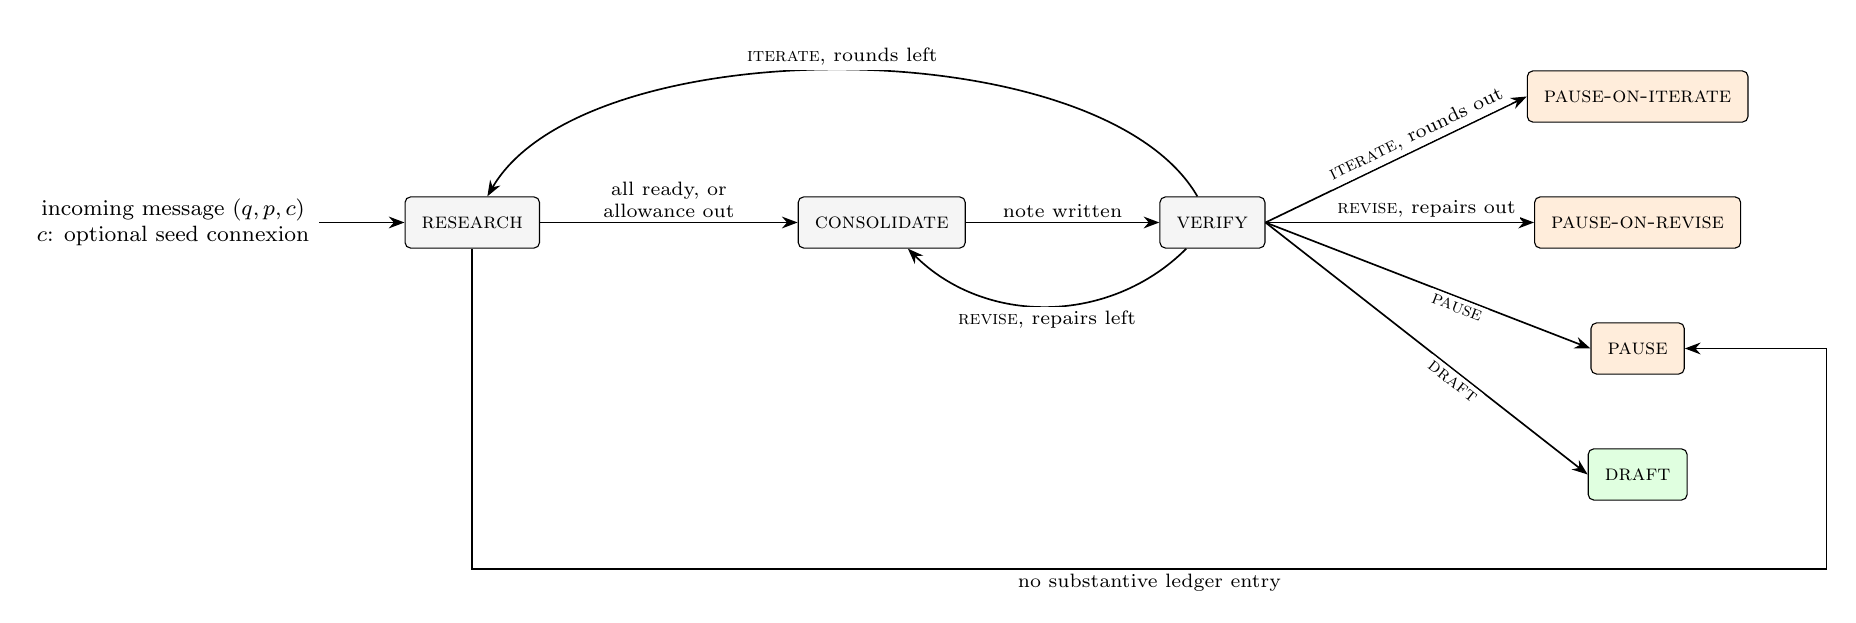
\begin{tikzpicture}[x=1cm,y=1cm, every node/.style={font=\footnotesize},
  state/.style={draw,rounded corners=2pt,minimum height=6.5mm,inner
  xsep=6pt,fill=gray!8}, term/.style={state,fill=green!12},
  pause/.style={state,fill=orange!14},
  edge/.style={-{Stealth[length=2mm]},semithick},
  lab/.style={font=\scriptsize,fill=white,inner sep=1.5pt}] \node[align=center]
  (input) at (2.4,0) {incoming message \((q,p,c)\)\\\(c\): optional seed
  connexion}; \node[state] (peers) at (6.2,0) {\st{research}}; \node[state]
  (cons) at (11.4,0) {\st{consolidate}}; \node[state] (ver) at (15.6,0)
  {\st{verify}}; \node[pause] (poi) at (21,1.6) {\st{pause-on-iterate}};
  \node[pause] (por) at (21,0) {\st{pause-on-revise}}; \node[pause] (pause) at
  (21,-1.6) {\st{pause}}; \node[term] (draft) at (21,-3.2) {\st{draft}};
  \draw[edge] (input) -- (peers); \draw[edge] (peers) --
  node[lab,above,align=center] {all ready, or\\allowance out} (cons);
  \draw[edge] (cons) -- node[lab,above] {note written} (ver); \draw[edge] (ver)
  to[out=120,in=60,looseness=0.7] node[lab,above] {\st{iterate}, rounds left}
  (peers); \draw[edge] (ver) to[out=225,in=315,looseness=1.0] node[lab,below]
  {\st{revise}, repairs left} (cons); \draw[edge] (ver.east) --
  node[lab,sloped,below,pos=0.6] {\st{draft}} (draft.west); \draw[edge]
  (ver.east) -- node[lab,sloped,below,pos=0.6] {\st{pause}} (pause.west);
  \draw[edge] (ver.east) -- node[lab,above,pos=0.6] {\st{revise}, repairs out}
  (por.west); \draw[edge] (ver.east) -- node[lab,sloped,above,pos=0.6]
  {\st{iterate}, rounds out} (poi.west); \draw[edge] (peers.south) -- (6.2,-4.4)
  -- node[lab,below] {no substantive ledger entry} (23.4,-4.4) |- (pause.east);
  \end{tikzpicture}}
\end{center}

\paragraph{Research.}
Upon receiving a tuple, the runner creates a directory for this investigation,
stores the papers and their metadata, and makes the seed available. It launches
the researcher agents concurrently, each with a prompt, tools, an allowance and
its own working directory. Each sees the papers, seed, whole ledger and its
partners' working files. It may write freely in its own directory; shared
findings, objections, corrections and intentions go into the ledger. The prompt
asks whether there is something publishable to say about the pair, not for a
quota of positive results. A continuation also exposes the verifier's feedback.

There is no turn-taking. An agent declares itself ready with the number of the
latest ledger entry it has read. Any subsequent substantive entry invalidates
that declaration. A researcher whose readiness still holds waits rather than
spending another call to repeat itself. The round ends when every researcher has
a valid readiness declaration, or when the available calls or time have been
used. Readiness need not mean agreement: unresolved disagreements must remain
explicit. If no substantive entry has been produced, the thread ends in
\st{pause}; otherwise it proceeds to consolidation.

Writing a ledger entry is a state change even though it does not move the
control position. For a permitted entry \(z\) by researcher \(a\),
\[
 (\sigma,M,b)\xrightarrow{\mathrm{append}(a,z)}
 (\sigma,M\oplus\mathrm{entry}(a,z),b),\qquad\rho=\st{research}.
\]
The update assigns the next ledger sequence number. A substantive entry
invalidates any readiness declaration preceding it; a declaration records the
position its author reports having read, not proof of comprehension. Let
\(\mathrm{Ready}(M)\) mean that every researcher holds a valid declaration,
\(\mathrm{HasWork}(M)\) that the ledger has a substantive entry, and
\(\mathrm{Out}(b)\) that the round's call or time allowance has ended. At a
runnable stage boundary,
\[
 \begin{gathered}
 \rho=\st{research},\qquad \mathrm{Ready}(M)\lor\mathrm{Out}(b),\\
 (\sigma,M,b)\xrightarrow{\mathrm{round\ closed}}
 (\sigma[\rho\leftarrow\rho'],M\oplus\mathrm{closure},b),\\
 \rho'=\begin{cases}
  \st{consolidate},&\mathrm{HasWork}(M),\\
  \st{pause},&\text{otherwise}.
 \end{cases}
 \end{gathered}
\]
The closure record states whether readiness or exhaustion ended the round. Usage
from calls that have returned is already included in \(b\).

\paragraph{Consolidate.}
The first researcher, an arbitrary but fixed choice, receives a new prompt and
writes the research note. It sees the ledger, the researchers' files, and any
previous note. Every claim must point to the ledger entries supporting it. The
note records what was asked, what holds, the objections and their disposition,
and what remains open. If the allowance ended before common readiness, it must
not manufacture agreement. On later research rounds it retains the earlier
results that still stand and incorporates the new work. On a repair it instead
addresses the verifier's corrections without opening a new line of research.
Writing the note enables \st{verify}.

For a returned, structurally usable synthesis \(n\), this is the rule
\[
 (\sigma,M,b)\xrightarrow{\mathrm{note\ written}(n)}
 (\sigma[\rho\leftarrow\st{verify}],M_n,b_n),
 \qquad\rho=\st{consolidate}.
\]
Here \(M_n\) contains the synthesis and its evidence references. Usability means
that the required artifact exists and can be supplied to the verifier, not that
its scientific claims have already been accepted.

\paragraph{Verify.}
A verifier that has taken no part in the research is called without tools. The
papers, ledger and note are supplied inline; evidence left only in a private
working file is not thereby available to this judge. Its reply contains a
decision and a reason, with an action when more work is requested:
\begin{itemize}
\item \st{draft}: a supported, non-obvious result warrants writing up.
\item \st{revise}: the ledger supports the result but the note misstates it; the
reply lists corrections that can be made from the existing record.
\item \st{iterate}: a promising direction has a specific gap the researchers can
address with their papers, derivations, tools and accessible literature; the
reply names the next task.
\item \st{pause}: no supported direction warrants more work now, or progress
requires unavailable data, experiments or access; the reply names what is
missing.
\end{itemize}
The verifier must not repeatedly demand an input the record already shows the
researchers cannot supply. The runner saves the verdict with a digest of the
note judged. A continuing verdict is also added to the ledger as feedback. An
unreadable verdict is retained for inspection and leaves the operation
\st{blocked}, not \st{pause}.

\paragraph{The iterate loop.}
Research starts at round one. On \st{iterate}, if the research-round cap has not
been reached, the runner increments that counter and returns to \st{research}.
The researchers keep their ledger and files and address the specified gap. If
the cap has been reached, the thread instead ends in \st{pause-on-iterate}. Thus
a request for further research is recorded even when it cannot be executed.

\paragraph{The revise loop.}
The repair counter starts at zero. On \st{revise}, if a repair remains, the
runner increments it and returns to \st{consolidate} with the corrections. The
rewritten note is verified again. Otherwise the ending is \st{pause-on-revise}.
Repairs have their own cap because rewriting supported material is different
from asking the researchers to investigate again. The reference implementation
counts repairs across the investigation; an iterate does not replenish them.

\paragraph{Verifier transition rules.}
Let \(\nu\) be a parsed verdict with its reason and, when required, action. Let
\(M_\nu\) save it with the judged note's digest and the feedback required for an
executed continuation, and let \(b_\nu\) include the call's receipt. The
complete automatic decision is
\[
 (\sigma,M,b)\xrightarrow{\nu}
 (\sigma[\rho\leftarrow\rho_\nu],M_\nu,b'),
 \qquad\rho=\st{verify},
\]
with \(\rho_\nu\) and \(b'\) determined by the following table.
\begin{center}
\begin{tabular}{llll}
\toprule
Decision in \(\nu\) & Guard & \(\rho_\nu\) & \(b'\) \\
\midrule
\st{draft} & true & \st{draft} & \(b_\nu\) \\
\st{pause} & true & \st{pause} & \(b_\nu\) \\
\st{iterate} & \(r<\bar r\) & \st{research} & \(b_\nu[r\leftarrow r+1]\) \\
\st{iterate} & \(r\geq\bar r\) & \st{pause-on-iterate} & \(b_\nu\) \\
\st{revise} & \(u<\bar u\) & \st{consolidate} & \(b_\nu[u\leftarrow u+1]\) \\
\st{revise} & \(u\geq\bar u\) & \st{pause-on-revise} & \(b_\nu\) \\
\bottomrule
\end{tabular}
\end{center}
The guards make explicit that \st{iterate} does not reset \(u\), while
\st{revise} does not advance \(r\). No automatic research transition leaves
\(T_R\). Output requests can nevertheless act on the other components of
\(\sigma\). An invalid reply does not match this table; the operational failure
rule below applies instead.

\section{The editing phase}

Research ends with an assessment of a connexion, not necessarily with a paper
ready for a reader. The editing phase has independent output branches. A
\st{draft} enables the \emph{paper} branch. Every terminal research outcome
enables the \emph{readable account} branch, whose purpose is to let an expert
assess what the research achieved and why it stopped. Neither branch is
authorised to change the research record.

Formally, an output request changes only its own component. For a fresh branch,
the launch rules are
\[
 \begin{gathered}
 \rho=\st{draft},\quad\pi=\st{idle}:\\
 (\sigma,M,b)\xrightarrow{\mathrm{request\ paper}}
  (\sigma[\pi\leftarrow\st{author}],M,b[w\leftarrow1]),\\[4pt]
 \rho\in T_R,\quad\eta=\st{idle}:\\
 (\sigma,M,b)\xrightarrow{\mathrm{request\ account}}
  (\sigma[\eta\leftarrow\st{editor}],M,b[e\leftarrow1]).
 \end{gathered}
\]
Both require a runnable branch, no stop request, and an available initial
attempt. The second rule has no condition on \(\pi\): an account can precede the
paper or be produced when no paper will be requested. Neither request changes
\(\rho\).

\begin{center}
\resizebox{\textwidth}{!}{%
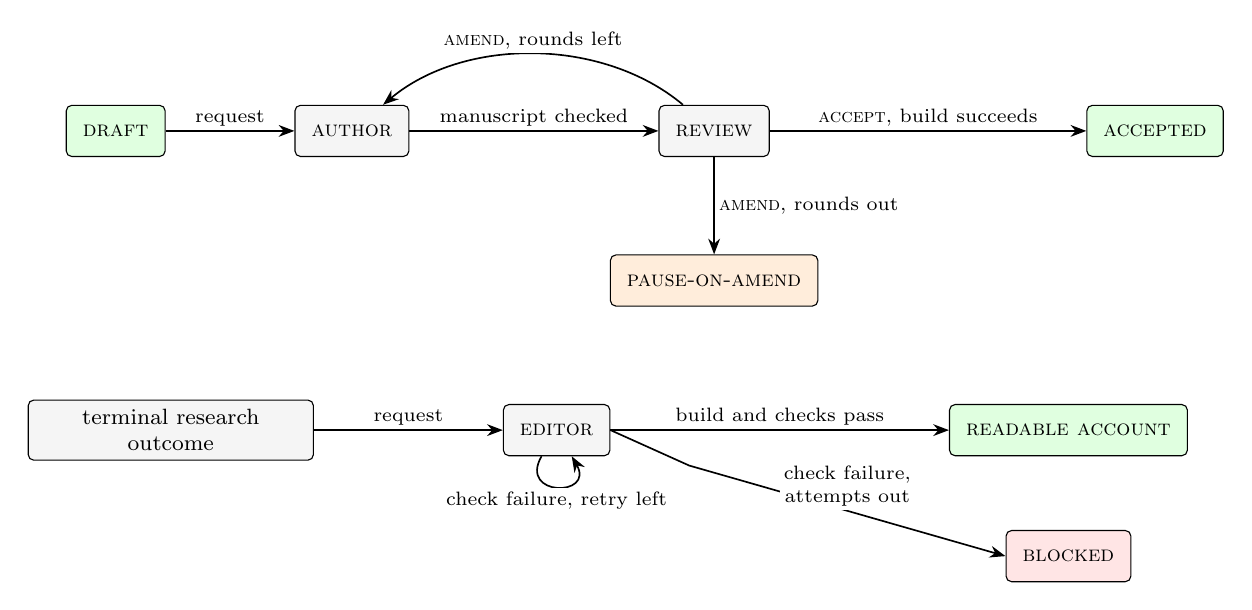
\begin{tikzpicture}[x=1cm,y=1cm, every node/.style={font=\footnotesize},
  state/.style={draw,rounded corners=2pt,minimum height=6.5mm,inner
  xsep=6pt,fill=gray!8}, term/.style={state,fill=green!12},
  pause/.style={state,fill=orange!14}, blocked/.style={state,fill=red!10},
  edge/.style={-{Stealth[length=2mm]},semithick},
  lab/.style={font=\scriptsize,fill=white,inner sep=1.5pt}] \node[term] (draft)
  at (0.8,0) {\st{draft}}; \node[state] (author) at (3.8,0) {\st{author}};
  \node[state] (review) at (8.4,0) {\st{review}}; \node[term] (accepted) at
  (14,0) {\st{accepted}}; \node[pause] (paused) at (8.4,-1.9)
  {\st{pause-on-amend}}; \draw[edge] (draft) -- node[lab,above] {request}
  (author); \draw[edge] (author) -- node[lab,above] {manuscript checked}
  (review); \draw[edge] (review) -- node[lab,above] {\st{accept}, build
  succeeds} (accepted); \draw[edge] (review) to[out=140,in=40,looseness=0.9]
  node[lab,above] {\st{amend}, rounds left} (author); \draw[edge] (review) --
  node[lab,right] {\st{amend}, rounds out} (paused);
  \node[state,align=center,text width=32mm] (terminal) at (1.5,-3.8) {terminal
  research\\outcome}; \node[state] (editor) at (6.4,-3.8) {\st{editor}};
  \node[term] (readable) at (12.9,-3.8) {\st{readable account}}; \node[blocked]
  (blocked) at (12.9,-5.4) {\st{blocked}}; \draw[edge] (terminal) --
  node[lab,above] {request} (editor); \draw[edge] (editor) -- node[lab,above]
  {build and checks pass} (readable); \draw[edge] (editor)
  to[out=240,in=300,looseness=4] node[lab,below] {check failure, retry left}
  (editor); \draw[edge] (editor.east) -- ++(1,-0.45) --
  node[lab,above,align=center,pos=0.5] {check failure,\\attempts out}
  (blocked.west); \end{tikzpicture}}
\end{center}

\paragraph{Author.}
The author receives the research note, ledger, verdicts, source papers and
researchers' working files. It has tools and web search. Its task is to turn the
supported material into a self-contained paper, not to add a theorem that the
research record does not establish. It distinguishes the source papers' results,
the contribution, interpretation, and limitations. It also searches for prior
work on the specific contribution, verifies reference metadata, and records what
it searched and found. Discovering that a construction is known changes its
attribution and claimed contribution; it is not a reason to conceal the
construction or its source.

\paragraph{Check.}
Once a manuscript and bibliography exist, the runner builds the paper and checks
its references. Cited keys must exist; bibliography entries must be cited and
carry identifying information. Where an arXiv lookup succeeds, its title is
compared with the bibliography. The build result and all findings are passed to
the reviewer. A lookup failure is reported as an unavailable check, not as
verification of the metadata. A failed build can still be reviewed for
correction, but cannot yield an accepted output.

Once a required manuscript exists and its checks have run, the transition is
\[
 (\sigma,M,b)\xrightarrow{\mathrm{manuscript\ checked}}
 (\sigma[\pi\leftarrow\st{review}],M_c,b_c),
 \qquad\pi=\st{author}.
\]
The update stores the manuscript, bibliography, search record, checks and
author-call receipt. The build need not succeed to enable review: a failed build
is evidence the reviewer can use. The check record identifies the version
checked so that a later acceptance cannot refer to a different one.

\paragraph{Review.}
The reviewer is a fresh call without tools. It receives the source papers,
research ledger and note, manuscript, bibliography, search record, and check
results. It asks whether the paper is fit to send to referees within its stated
scope: are its arguments supported and understandable, its attribution fair, and
its related-work claims justified by the record? The answer is \st{accept} or
\st{amend}, with an explanation and identified findings marked major or minor.
The runner saves the review with the manuscript's digest.

An \st{accept} may include minor corrections to wording or notation that do not
change a claim. \st{amend} requests changes to a claim, its scope, attribution
or correctness, or another defect that would obstruct assessment. This
distinction gives the loop a stopping rule: the target is an assessable
manuscript, not an absence of all possible editorial comments. Acceptance with
minor findings leaves those findings recorded; it does not imply they have
already been applied.

\paragraph{The amend loop.}
With rounds left, \st{amend} returns the paper to the author with the identified
findings. The author addresses each from the existing material and explains what
changed. The runner builds and checks the replacement before another review.
Each author--reviewer pass counts as a paper round. At the cap, unresolved
amendments lead to \st{pause-on-amend}. If a reviewer accepts a manuscript whose
build failed, acceptance is withheld and the remaining correction allowance is
used instead. Missing required files or an unreadable review are operational
blockages, not scientific rejections.

For a parsed review \(\mu\), define \(\mathrm{Acceptable}(\mu,M)\) to mean that
its decision is \st{accept} and the corresponding manuscript has a successful
build. Let \(M_\mu\) save the review, manuscript digest and findings, and
\(b_\mu\) account for the call. Then
\[
 (\sigma,M,b)\xrightarrow{\mu}
 (\sigma[\pi\leftarrow\pi_\mu],M_\mu,b'),
 \qquad\pi=\st{review},
\]
where
\[
 (\pi_\mu,b')=
 \begin{cases}
  (\st{accepted},b_\mu),&\mathrm{Acceptable}(\mu,M),\\
  (\st{author},b_\mu[w\leftarrow w+1]),
    &\neg\mathrm{Acceptable}(\mu,M),\ w<\bar w,\\
  (\st{pause-on-amend},b_\mu),
    &\neg\mathrm{Acceptable}(\mu,M),\ w\geq\bar w.
 \end{cases}
\]
Here the non-acceptable cases are \st{amend} or \st{accept} with a failed build,
not malformed replies. This rule counts automatic author--reviewer rounds; the
owner-directed reviewer-only workflow is described separately.

\paragraph{Readable account.}
After a terminal research outcome, an editor receives the research record and
writes for an expert who has not followed the ledger. It explains the question,
approach, supported outcome, unresolved objections, stopping reason and possible
next step. Its purpose is assessment of the research, including an unsuccessful
attempt, rather than advocacy for publication. It has file tools but no
configured web search and is not asked to conduct new research. The runner
builds the account and checks its references. A failed build or a blocking
reference defect is returned for a bounded correction attempt; failure after the
allowance leaves this branch \st{blocked}. Unavailable external lookups remain
disclosed warnings.

The account cannot be produced while the research is still running, \st{stopped}
or \st{blocked}. The research runner normally requests it automatically after a
terminal verdict, unless a stop has been requested. The owner can request a
deferred account later. It neither waits for paper acceptance nor changes the
research verdict, and its own failure does not invalidate the other branch.

Let \(\mathrm{AccountOK}(M_c)\) mean a successful build with no blocking
reference defect; an unavailable external lookup remains a warning. After an
editor attempt and its checks,
\[
 (\sigma,M,b)\xrightarrow{\mathrm{account\ checked}}
 (\sigma',M_c,b'),\qquad \eta=\st{editor},\quad\rho\in T_R,
\]
where \(\mathrm{AccountOK}(M_c)\) sets \(\eta'=\st{readable\ account}\).
Otherwise, \(e<\bar e\) keeps \(\eta'=\st{editor}\) and sets \(e'=e+1\); at the
cap it keeps the saved editor position and sets \(\omega_A'=\st{blocked}\). All
other control components are unchanged, and \(b'\) includes the attempt's usage.
For each editing transition, the research projection of the record obeys
\[
  M'\!\restriction_R=M\!\restriction_R.
\]
This projection contains the input, research ledger, synthesis and scientific
verdicts, not the output branch's own files or receipts. It states precisely
what it means for editing to leave the research outcome alone.

\section{The campaign and its operational control}

A \emph{thread} is an instance of the machine for an input tuple. A
\emph{campaign} supplies the corpora, candidate selection, resource settings and
a scheduler for several threads. An \emph{owner}, human or delegated, chooses
these settings and decides what to do with outputs and pauses. The scientific
transition rules are the same whether a thread is run alone or occupies a seat
in a campaign.

\paragraph{Admission.}
Fetching and scanning precede the machine described here. The scanner assigns a
score and possibly a seed connexion to candidate pairs; selection produces a
shortlist. A free seat and a passing budget guard permit the runner to admit a
shortlisted investigation. Its stored position determines whether to start
research or resume an unfinished stage. Terminal threads are not automatically
researched again. The corpora and shortlist can grow without restarting threads
already admitted. In the reference layout a campaign and pair identify a thread;
another independent attempt needs a separate campaign or record.

\paragraph{Shared memory.}
The ledger is an append-only sequence of attributed, numbered entries. Appends
are serialised, although the researchers work concurrently. Substantive entries
carry ideas, findings, objections, corrections or intentions; readiness and
review entries have the control roles described above. The record also contains
the current notes and manuscripts, judgement histories, saved positions and
resource receipts. Saving a judgement with an artifact digest identifies what
was judged. A digest does not recover an overwritten version: full replay would
additionally require retaining that version and its invocation context.

The contracts say which records each role can use and what it may change.
Researchers do not edit their partners' files; the editing branches leave the
research record alone; judges receive their evidence rather than acquiring
unrecorded evidence with tools. These are role contracts, not a claim that every
file permission enforces them. Model and prompt choices remain part of the run's
provenance.

\paragraph{Context and ledger access.}
Ledger freshness is part of the researchers' contract. Each researcher tracks
the sequence number \(k\) of the latest entry it has read and refreshes its view
before a major change of direction and before declaring readiness. A readiness
declaration names that observed position; it cannot certify unseen entries. Any
substantive entry after \(k\), including one appended between the refresh and
the declaration, makes that declaration stale. The runner determines common
readiness from the ledger, not from an agent's unqualified statement that it has
finished.

Incremental reading is a recommended implementation refinement. A ledger helper
may return only entries after \(k\), in sequence order, together with the
position reached; the researcher advances its cursor after reading them. This
avoids repeatedly supplying material already available in the current
invocation. A cursor alone is not a substitute for that material: a fresh
invocation must receive the existing ledger before consuming subsequent updates.
After context compaction, the agent must retain or reload the earlier evidence
needed for its next claim; the cursor does not establish that this evidence
remains available. A full refresh is the safe fallback. These rules do not
require incremental retrieval in the reference helper.

Prefix sharing is a separate execution optimisation. Within the shared task
context, the current implementation places the source papers first, followed by
the growing ledger, before caller-specific instructions and changing material.
Judges also receive the note being assessed. An implementation should preserve
the common material and its ordering between calls, placing unnecessary per-call
variation outside the reusable prefix. The backend must configure any required
cache boundaries and report actual cache usage rather than infer a cache hit
from shared text. Provider-specific cache settings do not belong to the
transition system. Every call must still supply its required context, whether
directly or through the backend's supported context mechanism; correctness and
ledger freshness must never depend on a cache hit.

\paragraph{Allowances.}
The resource settings attach to different loops and should not be conflated.
\begin{center}
\begin{tabularx}{\textwidth}{@{}lXX@{}}
\toprule
Allowance & Scope & Exhaustion effect \\
\midrule
Researcher calls and time & A research round & Consolidate the existing ledger.
\\
Research rounds & The iterate loop & \st{pause-on-iterate}. \\
Note repairs & The revise loop & \st{pause-on-revise}. \\
Paper rounds & The amend loop & \st{pause-on-amend}. \\
Account attempts & Build and reference repair & The account is \st{blocked}. \\
Campaign expenditure & Admission of threads & Stop new admission. \\
\bottomrule
\end{tabularx}
\end{center}
Each model call also has a deadline. The reference defaults allow four research
rounds, one note repair, three paper rounds and two account attempts; these
numbers are settings, not properties of the scientific task. Within a research
round the call cap applies per researcher and elapsed call time is accumulated
across researchers.

Calls append receipts recording the usage reported by the provider and the
available cost estimate. The admission guard compares recorded expenditure plus
a reservation for work in flight against the campaign budget. This is a
scheduling guard, not a strict upper bound on the eventual bill: admitted
threads can need further calls, and concurrent researchers can overshoot a
shared time allowance before their usage is collected. Token usage is recorded,
but the present runner does not enforce a separate hard token quota. Unpriced
subscription usage must not be interpreted as free work. Strict reservation
before every call would require a stronger accounting mechanism.

\paragraph{Stop.}
A stop request prevents new admission and is tested at call or stage boundaries.
Calls already in flight are allowed to return, and their work is recorded. A
thread that has not reached a terminal verdict keeps its current stage and
becomes \st{stopped}. Clearing the request permits continuation from that stage.
It does not require finishing the whole investigation before the runner stops,
and it does not turn an interruption into \st{pause}.

The operational mode makes this distinction explicit. For a branch \(j\) that
still has work, at a safe boundary,
\[
 (\sigma,M,b)\xrightarrow{\mathrm{stop\ boundary}_j}
 (\sigma[\omega_j\leftarrow\st{stopped}],M,b).
\]
The stage positions \(\rho,\pi,\eta\) are unchanged. No new call is launched
while its branch is not runnable or a stop request is pending. An in-flight call
may still return and record its result and usage; the stop guard is applied
before launching further work. An account request is therefore deferred, not
enabled merely because research was interrupted.

\paragraph{Failure and recovery.}
Failure to establish a model session is a transport failure: the scientific
decision has not been made. The thread is stopped; repeated transport failures
pause campaign admission until a probe succeeds. A call that starts but times
out may already have written useful files. Recovery therefore considers both the
saved position and the required artifacts, rather than treating every timeout as
a fresh investigation. Bounded call retries are distinct from the verifier's
requests for new research.

A blocked operation has no usable contracted output, for example an unreadable
verdict, and waits for inspection. Reconciliation chooses the next operational
step: resume research, consolidate, or verify an existing note. It does not
invent a scientific verdict. The implementation saves files and positions
separately, so a crash between them can require repeating a call. Researcher
time and call counters within a round are not durable across every restart. The
guarantee is preservation of recorded work, not exactly-once execution or an
unchanged remaining allowance after arbitrary failures.

For example, a returned but unparsable judge reply \(z\) has the rule
\[
 (\sigma,M,b)\xrightarrow{\mathrm{bad\ reply}_j(z)}
 (\sigma[\omega_j\leftarrow\st{blocked}],M_z,b_z).
\]
It records the raw reply and usage but supplies no \st{draft}, \st{pause},
\st{accept}, or \st{amend} label. A transport failure instead marks the
unfinished branch \st{stopped} and records the failure. A resume or
reconciliation event can restore \st{runnable} only after the stop or failure
condition has been addressed and the saved artifacts identify a usable
continuation. These operational events do not manufacture a scientific verdict
or silently start a new independent investigation.

\paragraph{Owner intervention.}
A terminal research outcome ends that automatic run. Raising an allowance alone
does not reopen it in the reference implementation. The owner can supply missing
evidence and start a separately recorded investigation, or arrange an explicit
continuation while retaining the old outcome. For a paper paused on amendments,
increasing the paper-round cap permits further author--reviewer passes.
Alternatively, the owner can edit it and request a reviewer-only pass; this
counts as another review without an author call and can exceed the automatic
round cap. These manual calls still consume resources, even though the admission
guard does not bound that workflow.

The runner uses a per-thread ownership marker to avoid ordinary duplicate
admission. Independent paper or editor commands must also be serialised by the
owner; the reference runner's marker is not a general transactional lock
covering every command. A stronger implementation can enforce these ownership
rules without changing the scientific states.

\section{What the process establishes}
\label{sec:establishes}

The machine separates proposing a connexion, supporting it, and presenting it
for assessment. \st{draft} means that the verifier found enough supported
material to justify writing. \st{accepted} means that the internal paper
reviewer found the manuscript assessable within its stated scope. Neither label
certifies scientific truth, exhaustive novelty, or eventual acceptance by a
journal. Conversely, a pause can be informative: its account should identify a
failed construction, a missing input, or a precise limit on what the current
materials support.

Independent calls provide a separation of roles, not independence of every model
error. A shared misconception can pass through researchers and judges.
Correctness, novelty and significance remain questions for the expert reader,
who can inspect the sources, arguments and limitations. This is why the readable
account is an output in its own right, rather than merely a by-product of
successful paper writing.

An implementation of this description should preserve the guarded transitions,
the evidence available to each role, the distinction between scientific and
operational endings, and the records needed to explain each decision. It need
not reproduce the same model responses. Pathfinder organises attempts at
scientific discovery; it does not make their outcome deterministic.

The notation also exposes useful invariants of the automatic machine:
\[
 \begin{aligned}
 \eta\in\{\st{editor},\st{readable\ account}\}
    &\ \Longrightarrow\ \rho\in T_R,\\
 \pi\ne\st{idle}
    &\ \Longrightarrow\ \rho=\st{draft},\\
 \pi=\st{accepted}
    &\ \Longrightarrow\ \text{an accepting review and successful build}\\
    &\hspace{28mm}\text{identify the same manuscript version.}
 \end{aligned}
\]
They follow from the launch and completion guards, preservation of the research
record by editing, and the absence of an automatic transition out of a terminal
research position. Stops and blockages change operational modes, not these
scientific prerequisites. Explicit owner continuations must preserve their prior
outcomes and provenance rather than be confused with an automatic edge in the
original run.

\appendix
\section{Agent resources against human resources, per pair}
\label{app:resources}

The economics has several distinct measures: tokens consumed, model charges,
elapsed time, and human attention. The root campaign used $330$ model calls
with $186.58$~USD of recorded charges; its outcomes and mixed-model setup are
described in Section~\ref{sec:pilot}. Later reruns and repairs are excluded.
The recorded activity spans 11--13 September, including interruptions and
owner-directed continuations, rather than an uninterrupted benchmark run.

\paragraph{Agent resources.}
Table~\ref{tab:agent-resources} carries over the approximate per-stage figures
from the original campaign summary. That summary reports typical costs and
times as medians over threads, with the qualifications shown below. These
figures have not been recomputed here from individual call intervals and
should not be added to obtain a measured end-to-end median. Dollar amounts
use the historical accounting rates, not a common GPT-6 price basis.

\begin{table}[htbp]
\centering
\small
\begin{tabularx}{\linewidth}{@{}Xrrl@{}}
\toprule
Stage, per pair & Calls & USD & Elapsed time \\
\midrule
Scan & 1 & 0.03 & 11 s \\
Research, consolidation and verification & 12 & 6.8 & 8 min \\
Manuscript preparation and review & 4--11 & 3.5 & 5 min per round \\
Readable account & 1 & 1.0 & 2 min \\
\bottomrule
\end{tabularx}
\caption{Approximate figures retained from the original campaign summary.
Research was reported to average $9.8$~USD and $51$ minutes, with a worst
thread around $30$~USD and six hours. The longest manuscript sequence used
seven review rounds, with a reported cost of $14.7$~USD. These are descriptive
figures from a development campaign, not controlled performance estimates.}
\label{tab:agent-resources}
\end{table}

\paragraph{Tokens and a common price basis.}
The original summary does not give token totals, and dollar amounts cannot
be converted back into token counts without their breakdown. Repricing a
campaign requires separate counts for uncached input, cache reads, cache
writes, and billed output including reasoning. GPT-6 Astra's standard API
rates on 16 September 2026 are respectively $10$, $1$, $12.50$, and $50$~USD
per million tokens for requests of at most $272{,}000$ input tokens; above
that threshold the corresponding rates are $20$, $2$, $25$, and $75$~USD for
the full request.\footnote{OpenAI's published pricing and context threshold:
\url{https://developers.openai.com/api/docs/models/gpt-6-astra} and
\url{https://developers.openai.com/api/docs/pricing}.}
A common-price comparison would apply those rates to the recorded token
categories, retaining any separately billed tools. It would be a
\emph{GPT-6-equivalent token cost}, not an observed GPT-6 run. Choosing medium
reasoning effort does not determine how many tokens a rerun would consume.
Subscription charges and quota usage are separate measures, not zero-cost API
usage. No normalised campaign total is asserted here.

\paragraph{An illustrative human comparison.}
Table~\ref{tab:human-resources} retains the original note's estimates for a
postdoctoral-level researcher, valued at an assumed fully loaded rate of
$60$~USD per hour. These are workload assumptions, not observations from a
human control group or claims about prevailing salaries. They describe similar
stages of work, not demonstrated equality of scientific quality.

\begin{table}[htbp]
\centering
\small
\begin{tabularx}{\linewidth}{@{}Xrr@{}}
\toprule
Human activity, per pair & Hours & USD at $60$/h \\
\midrule
Read two abstracts and decide & 0.25 & 15 \\
Read both papers, investigate and write a research note & 25--40 & 1,500--2,400 \\
Colleague checks the research note & 2--4 & 120--240 \\
Prepare a paper with related-work search & 60--80 & 3,600--4,800 \\
Review the paper & 4--8 & 240--480 \\
Write a readable account & 4 & 240 \\
\bottomrule
\end{tabularx}
\caption{Illustrative human effort from the original note. A total would
require deciding how much research, literature search and writing overlap
between stages. Calendar time also depends on availability and review delays.}
\label{tab:human-resources}
\end{table}

Under the scanning assumption alone, examining $100$ pairs takes $25$ human
hours, compared with $3.34$~USD of recorded scan charges. This illustrates
why broad searches become affordable; it does not establish a quality-matched
speedup. A human researcher would normally select promising papers rather
than inspect every pair, and that selection is itself part of the expertise
being compared.

Human effort does not disappear from an agent campaign. The original account
estimated $10$--$20$ minutes of owner attention per pair, plus about an hour
for a manuscript requiring manual intervention; this was not a time-tracked
measurement. Reading and checking the scientific outputs remain necessary.
The potential saving is in moving human effort from producing every candidate
to selecting, assessing and developing promising ones, not in replacing
scientific assessment with internal acceptance.

Finally, elapsed time is not the sum of agent call durations. Researchers
overlap within a round, stages follow one another, and several threads may
run concurrently. Timeouts, queueing and pauses can dominate the calendar.
Cost, active computation time, campaign elapsed time and human attention
should therefore be reported separately. Neither the historical timing
figures nor the human estimates justify a general multiplier for speed or
cost advantage at equal scientific quality.

\section{Conformance tests for a reimplementation}
\label{app:conformance}

Scientific outputs cannot check a reimplementation, because the model responses
are not deterministic and need not agree between runs. What is checkable is the
transition system: the guards, the counters and their caps, the terminal labels,
and the separation of operational from scientific endings. These can be tested
without spending model calls.

The reference implementation does so with a substitute agent command driven by
environment variables: what to reply, how long to wait before announcing a
session, whether to hang instead of replying, and a shell command to run in the
working directory before replying. The substitute must write every file a real
call writes. Otherwise a branch that real calls never reach will pass.

The following paths exercise the specification above, and a reimplementation
that passes them may be considered faithful to it.
\begin{itemize}
\item A scan interrupted and resumed, and an unparsable scored row retried.
\item Selection by percentage cut, and by threshold with already started
investigations retained.
\item A thread reaching each of \st{draft}, \st{pause}, \st{pause-on-iterate}
and \st{pause-on-revise}.
\item The iterate cap, reached with the verifier still requesting research.
\item A repair applied once and the repair cap reached thereafter.
\item An empty ledger ending the thread in \st{pause}.
\item A stop request draining a call in flight, and a resume continuing from the
recorded stage.
\item The admission guard writing the stop marker when the budget is reached.
\item Two consecutive transport failures setting the health marker, and a
successful probe call clearing it.
\item Both blocked paths, an unreadable verdict and an unreadable review, and
reconciliation naming and applying the one safe action.
\item A killed runner leaving an ownership marker whose process is gone.
\item Append-only paging in open-ended mode, with existing pair identifiers
unchanged.
\item The paper and readable-account round trips against a real LaTeX build.
\end{itemize}

The invariants stated at the end of Section~\ref{sec:establishes} can be
asserted directly over the saved records while these tests run.

After they pass, a pilot on two corpora of about five papers a side, with stop,
resume and reconciliation exercised by hand, establishes what a campaign costs
and how long it takes before a larger one is attempted.

\section{Correspondence with the reference implementation}

The following names connect the description to the repository without making the
directory layout part of the mathematical state space. The pair identifier is
local to a campaign. Each role's prompt supplies the scientific criteria
described in the corresponding transition paragraph.

\begin{center}
\small
\begin{tabularx}{\textwidth}{@{}lX@{}}
\toprule
Record or operation & Reference representation \\
\midrule
Input papers and metadata & \file{threads/<pair>/inputs/}; the optional seed is
taken from the campaign scan. \\
Research record & \file{ledger.jsonl}, researcher directories and
\file{<pair>.tex}. \\
Research position and judgements & \file{status.json} and
\file{<pair>.verdict.json}. \\
Paper branch & \file{paper/}, including the manuscript, bibliography, search
record, checks and reviews. \\
Readable account & \file{edited/}, with its source, bibliography, PDF and
attempt status. \\
Campaign control & Shortlist, configuration, receipts, stop marker and health
marker. \\
Role instructions & \file{peer.md}, \file{consolidate.md}, \file{verify.md},
\file{author.md}, \file{review.md}, \file{editor.md}. \\
\bottomrule
\end{tabularx}
\end{center}

The verifier's structured reply has fields \file{decision}, \file{reason} and
\file{action}; the last carries corrections or the next research task, and is
otherwise empty. The paper reviewer returns \file{decision}, \file{summary} and
\file{findings}; each finding has an identifier, severity, location, issue and
proposed fix. The runner, rather than the judge, adds counters, timestamps and
artifact digests. State labels are rendered uniformly in this note; their
capitalisation and file-field names in the repository are serialization details.

\begin{thebibliography}{9}
\bibitem{swanson1986}
Don R. Swanson. Undiscovered public knowledge. \emph{The Library Quarterly},
56(2):103--118, 1986. \url{https://doi.org/10.1086/601720}.

\bibitem{gentner1983}
Dedre Gentner. Structure-mapping: A theoretical framework for analogy.
\emph{Cognitive Science}, 7(2):155--170, 1983.
\url{https://doi.org/10.1207/s15516709cog0702_3}.
\end{thebibliography}

\end{document}
